\section{Análisis y preprocesado de los datos}

\subsection{Análisis del conjunto de datos}

Nuestro conjunto de datos se compone de tres ficheros:

\begin{enumerate}
	\item \texttt{lateralidad0.arff} : 473 muestras de la lateralidad izquierda del pubis.
	\item \texttt{lateralidad1.arff} : 487 muestras de la lateralidad derecha del pubis.
	\item \texttt{completo.arff} : 960 muestas de ambas lateralidades, se compone de los dos ficheros antes en conjunto.
\end{enumerate}

\begin{figure}[H]
	\begin{lstlisting}[language={}]
	NoGrooves,Absence,Defined,Absent,Defined,Present,Absent,Absent,FormedWithoutRarefactions,Ph07-35-39
	\end{lstlisting}
	\caption{Ejemplo de un dato cuya edad de muerte está en el rango comprendido por la fase 7, entre 35 y 39 años, del conjunto de datos \texttt{completo.arff}.}
	\label{fig:ejemplo_dato}
\end{figure}

Como vemos en la figura \ref{fig:ejemplo_dato} los datos tienen asignados valores categóricos para cada característica, y finalmente la edad a la que murió la persona con las características asociadas.

Para comenzar, realizaremos un análisis de cada uno de los conjuntos de datos. Como el conjunto de datos completo se trata simplemente de la unión de los datos de la lateralizad izquierda y la derecha, será el último análisis que realicemos.

\subsubsection{Análisis del conjunto de datos completo}

El conjunto completo de los datos cuenta con 960 observaciones, las de la lateralidad izquierda y derecha unidas.

\begin{figure}[H]
	\centering
	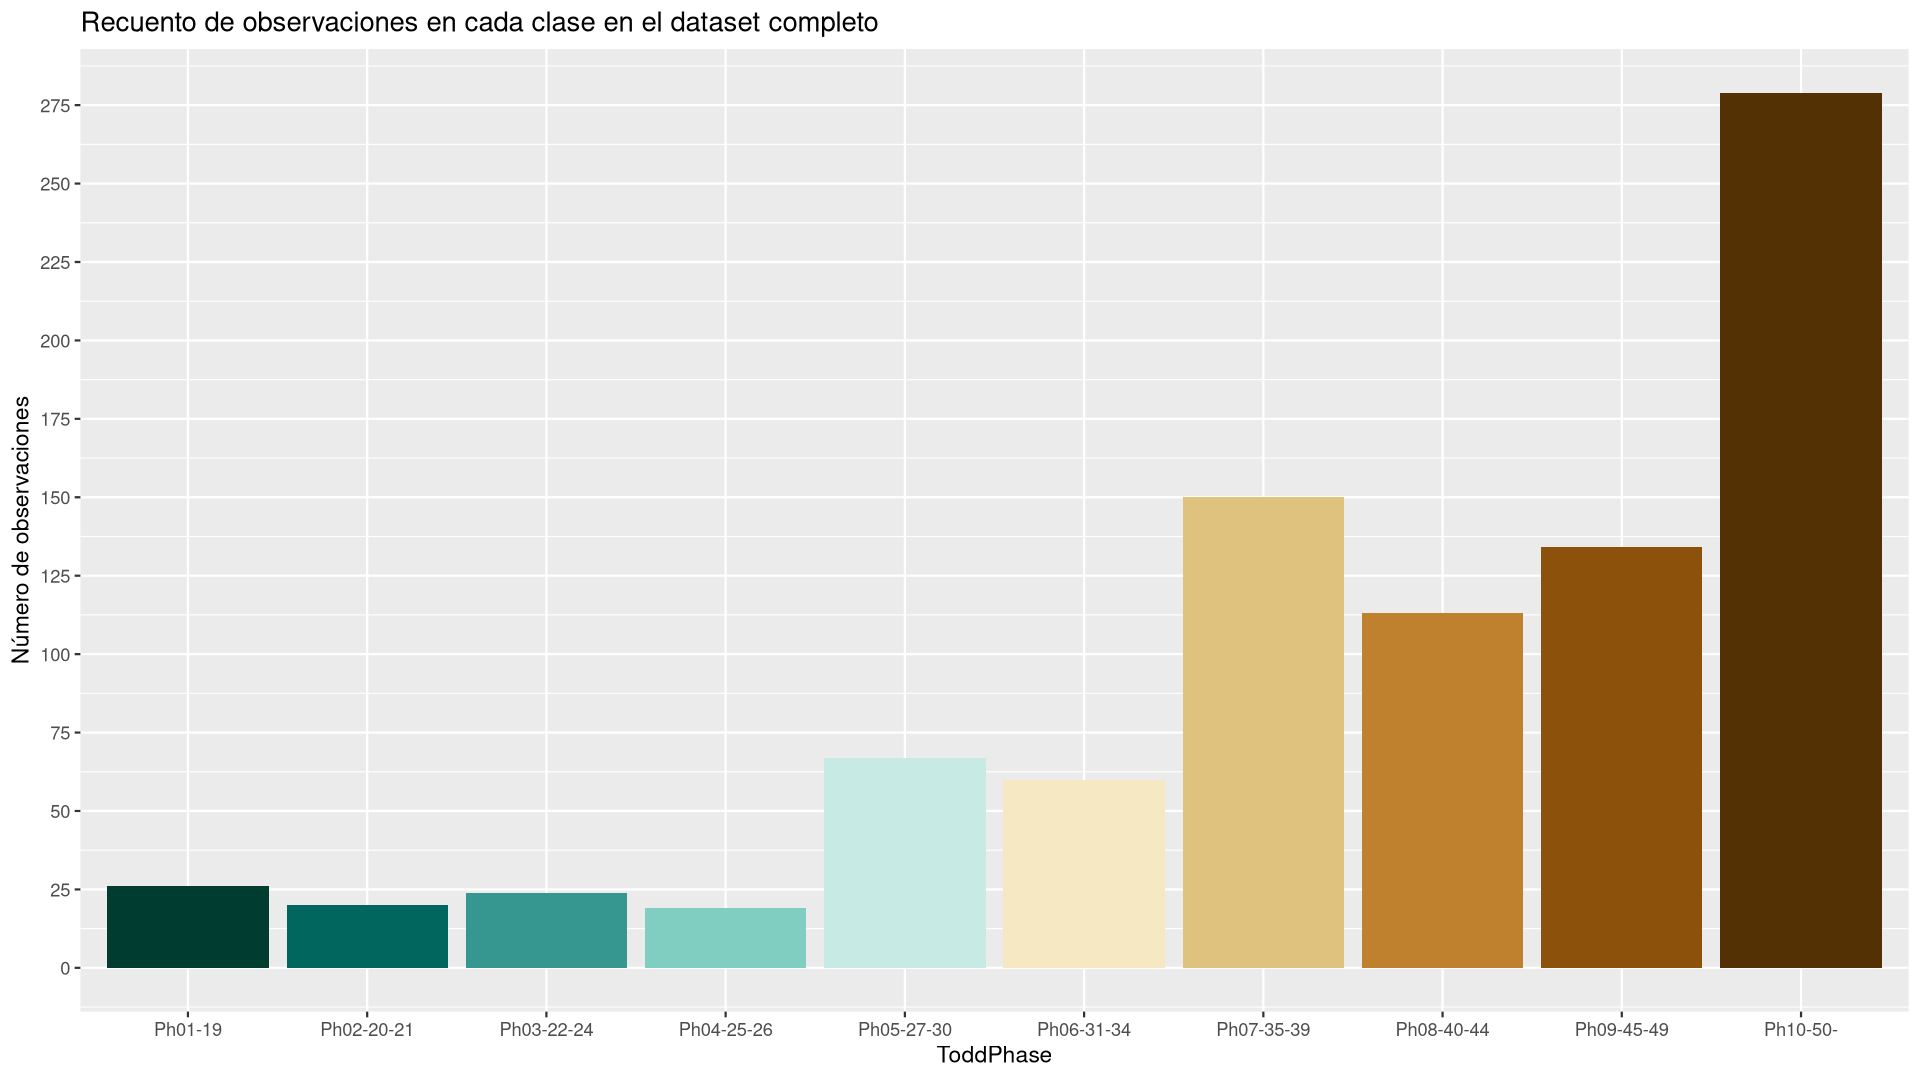
\includegraphics[width = \textwidth]{conjunto_datos/distribucion_clases_completo.png}
	\caption{Número de datos por cada fase propuesta por Todd con el conjunto de datos completo.}
	\label{fig:conteo_c}
\end{figure}


Podemos ver que contamos con una cantidad muy alta de observaciones de las últimas fases en comparación con las primeras fases, en especial de la última fase, de personas de más de cincuenta años.

Debido a que todas las variables del conjunto de datos son categóricas, para este análisis solo podemos observar como se distribuyen los valores de cada predictor para cada fase. Vamos ver cada uno de estos predictores y comentar la información que nos proporcionan.


\begin{figure}[H]
	\centering
	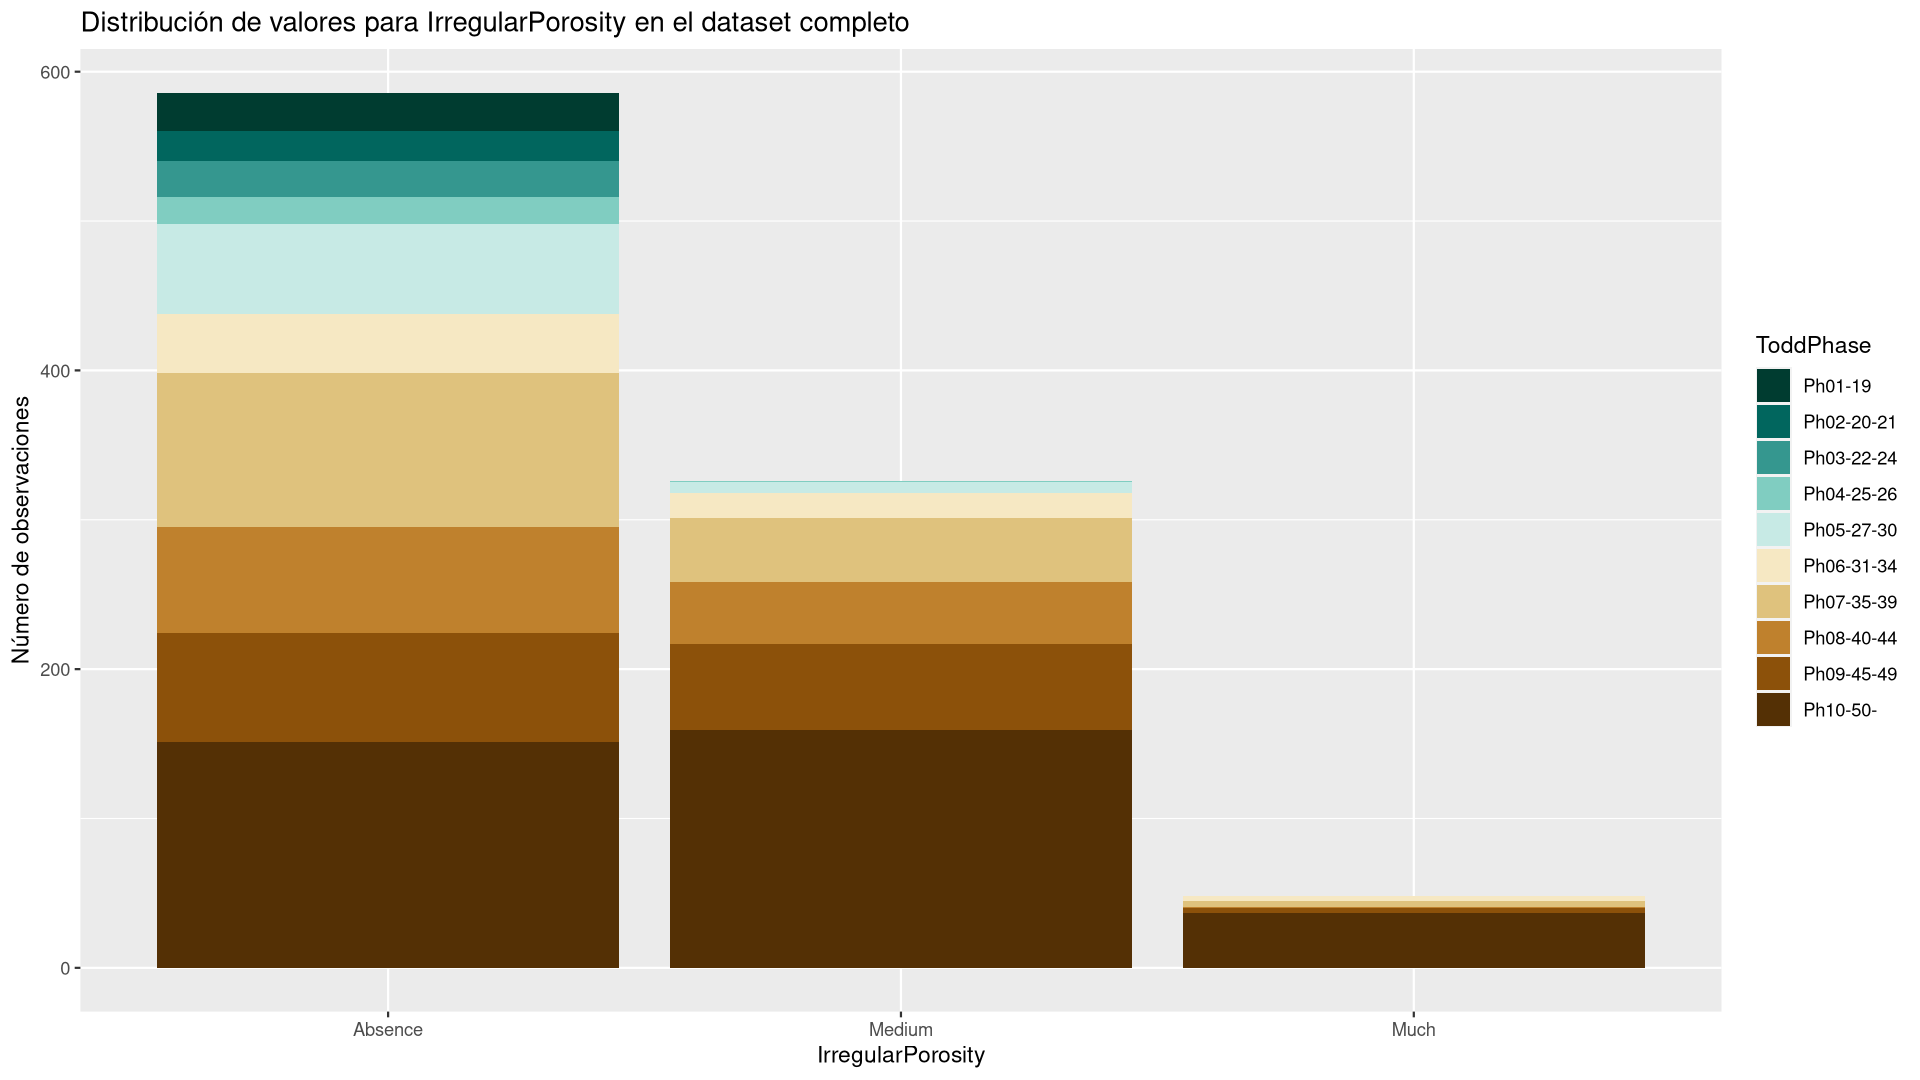
\includegraphics[width = \textwidth]{conjunto_datos/densidad_IrregularPorosity_completo.png}
	\caption{Distribución de los valores de IrregularPorosity en el conjunto de datos completo.}
	\label{fig:densidad_IrregularPorosity_completo}
\end{figure}

En la figura \ref{fig:densidad_IrregularPorosity_completo} podemos observar la distribución de valores de \texttt{IrregularPorosity}. En este vemos como claramente con esta característica podremos clasificar observaciones de fases altas si el valor de esta variable es \texttt{Much}, mientras que con el valor \texttt{Medium} y en especial \texttt{Absence} si hay un mayor solapamiento entre las clases.

Aun así, podemos ver como esta característica tampoco nos aporta gran información para las fases más bajas, donde si se solapa este valor. Vamos a seguir observando el resto de predictores.




\begin{figure}[H]
	\centering
	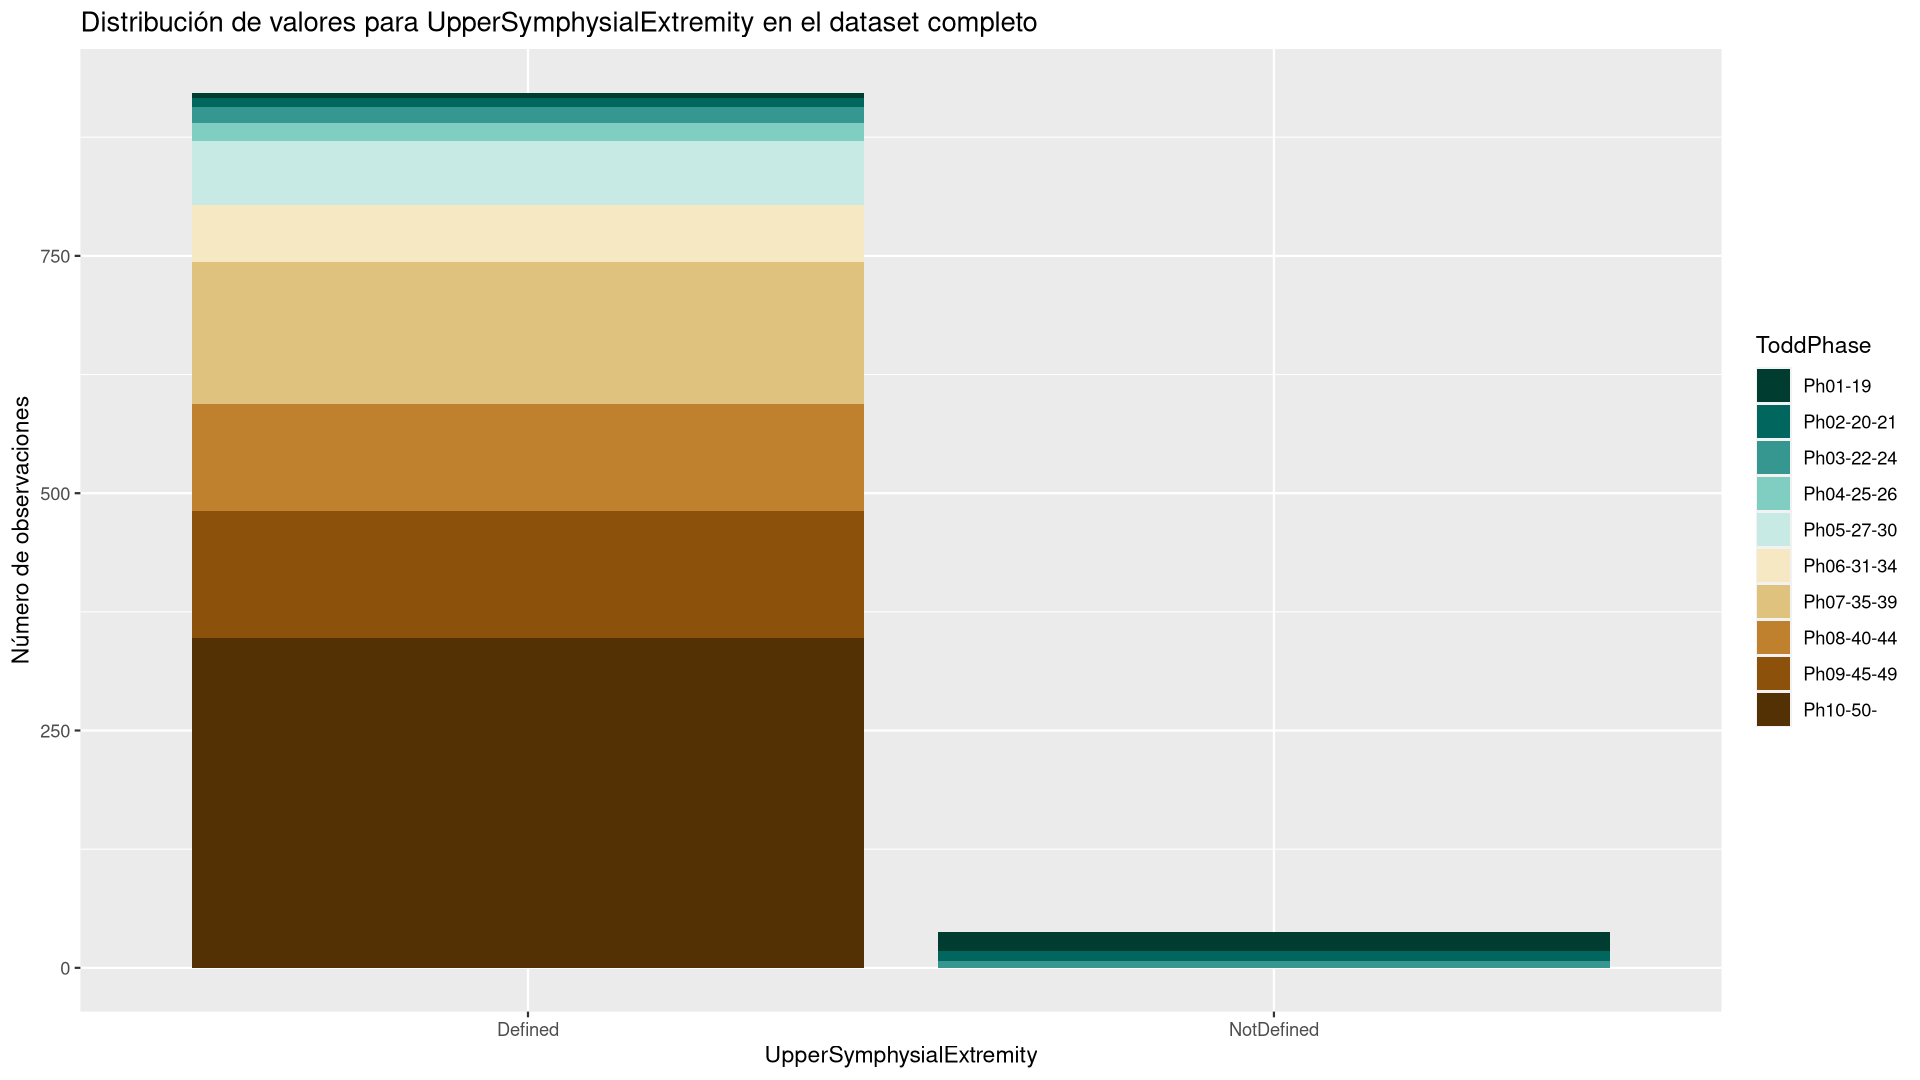
\includegraphics[width = \textwidth]{conjunto_datos/densidad_UpperSymphysialExtremity_completo.png}
	\caption{Distribución de los valores de UpperSymphysialExtremity en el conjunto de datos completo.}
	\label{fig:densidad_UpperSymphysialExtremity_completo}
\end{figure}

En este caso con \texttt{UpperSymphysialExtremity}, como vemos en la figura \ref{fig:densidad_UpperSymphysialExtremity_completo}, ocurre lo contrario que en el caso anterior. Esta característica nos podría servir muy bien para predecir asegurarnos que estamos ante observaciones de fases bajas si toma el valor de \texttt{NotDefined}, sin embargo vemos como las observaciones con este valor siguen existiendo tres posibles clases, por lo que realmente no hemos resuelto por completo estas observaciones, pero si acotado bastante el rango de fases, al ser tres contiguas.


\begin{figure}[H]
	\centering
	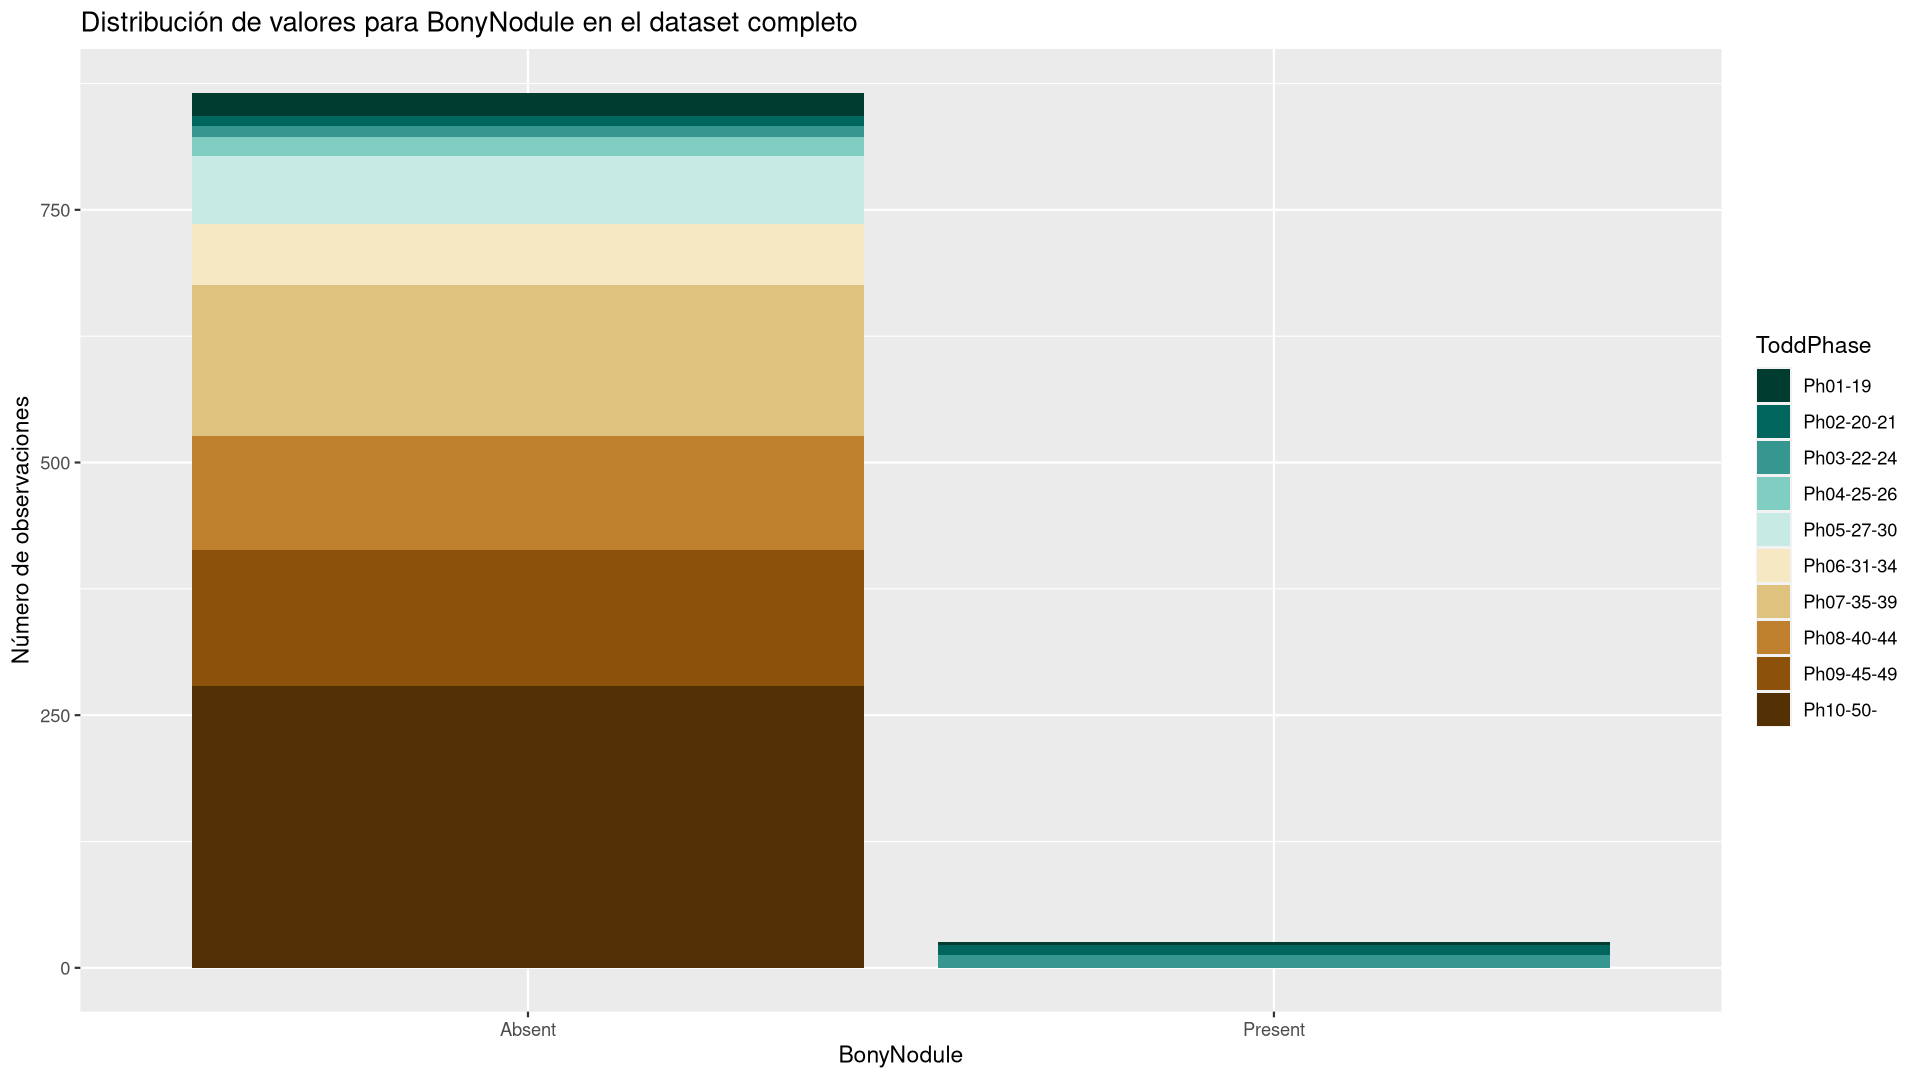
\includegraphics[width = \textwidth]{conjunto_datos/densidad_BonyNodule_completo.png}
	\caption{Distribución de los valores de BonyNodule en el conjunto de datos completo.}
	\label{fig:densidad_BonyNodule_completo}
\end{figure}

Para la variable \texttt{BonyNodule} ocurre lo mismo que con la variable anterior, \texttt{UpperSymphysialExtremity}. Cuando se toma el valor de \texttt{Present} vemos como todas las observaciones son de fases bajas, aunque sigue existiendo ciertas dudas sobre la fase concreta. Cuando toma el valor de \texttt{Absent} no se puede sacar ninguna conclusión debido a que encontramos valores de todas las clases.



\begin{figure}[H]
	\centering
	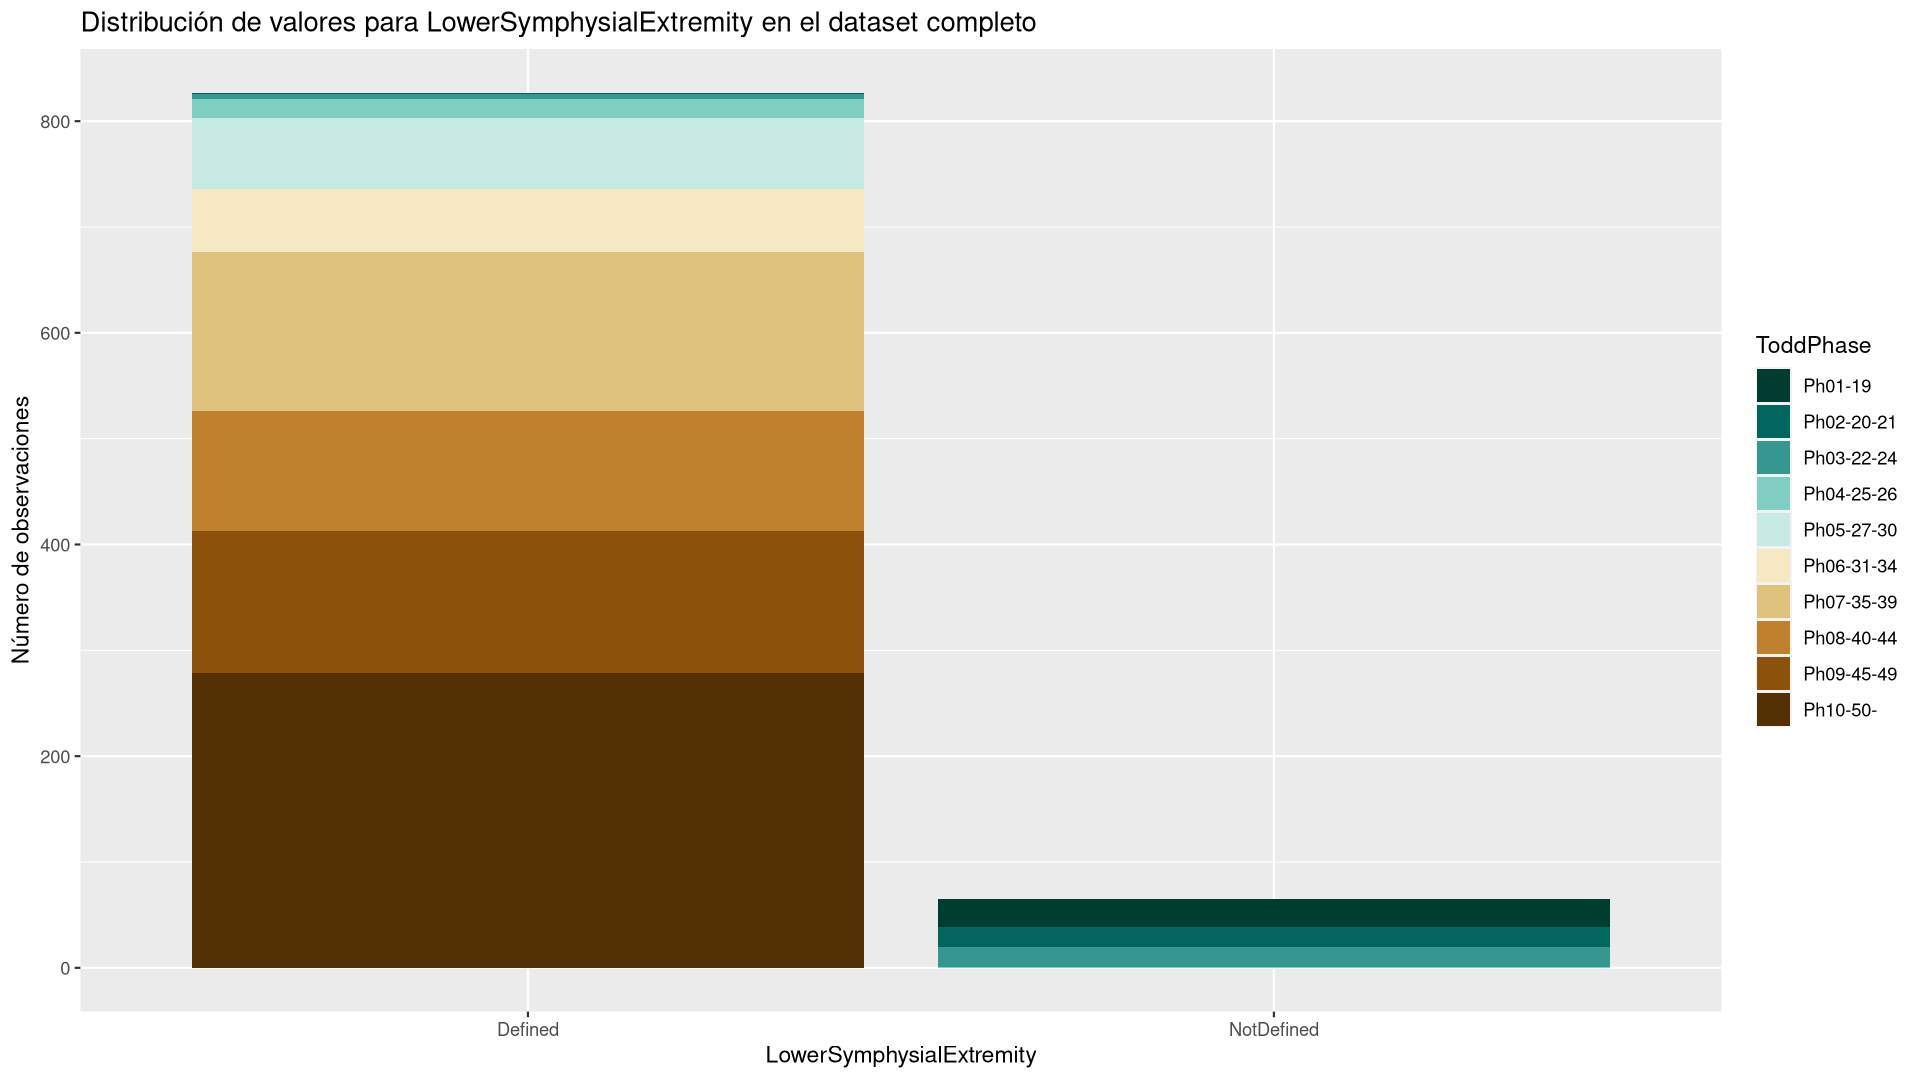
\includegraphics[width = \textwidth]{conjunto_datos/densidad_LowerSymphysialExtremity_completo.png}
	\caption{Distribución de los valores de LowerSymphysialExtremity en el conjunto de datos completo.}
	\label{fig:densidad_LowerSymphysialExtremity_completo}
\end{figure}

Con \texttt{LowerSymphysialExtremity} se puede observar que ocurre al igual que en casos anteriores, si toma el valor \texttt{NotDefined} podemos ver que se trata de una fase baja, sin embargo, en este caso si que nos llega a aportar algo más de información. En los casos anteriores, aunque un valor nos discriminaba muy bien si era de una fase temprana o no, el valor contrario seguía teniendo valores de todas las clases, es decir, si por ejemplo \texttt{BonyNodule} toma el valor \texttt{Present}, sabemos que se trata de una fase temprana, sin embargo si toma el valor \texttt{Absent} no podemos decir nada, porque podría ser de cualquier fase, sin embargo, con \texttt{LowerSymphysialExtremity} podemos ver claramente como si es \texttt{NotDefined} será de una clase baja, pero si es \texttt{Defined} podemos concluir que, al menos de la primera fase no será esta observación, ya que no encontramos observaciones de esta fase, y muy pocas de la fase dos y tres.

\begin{figure}[H]
	\centering
	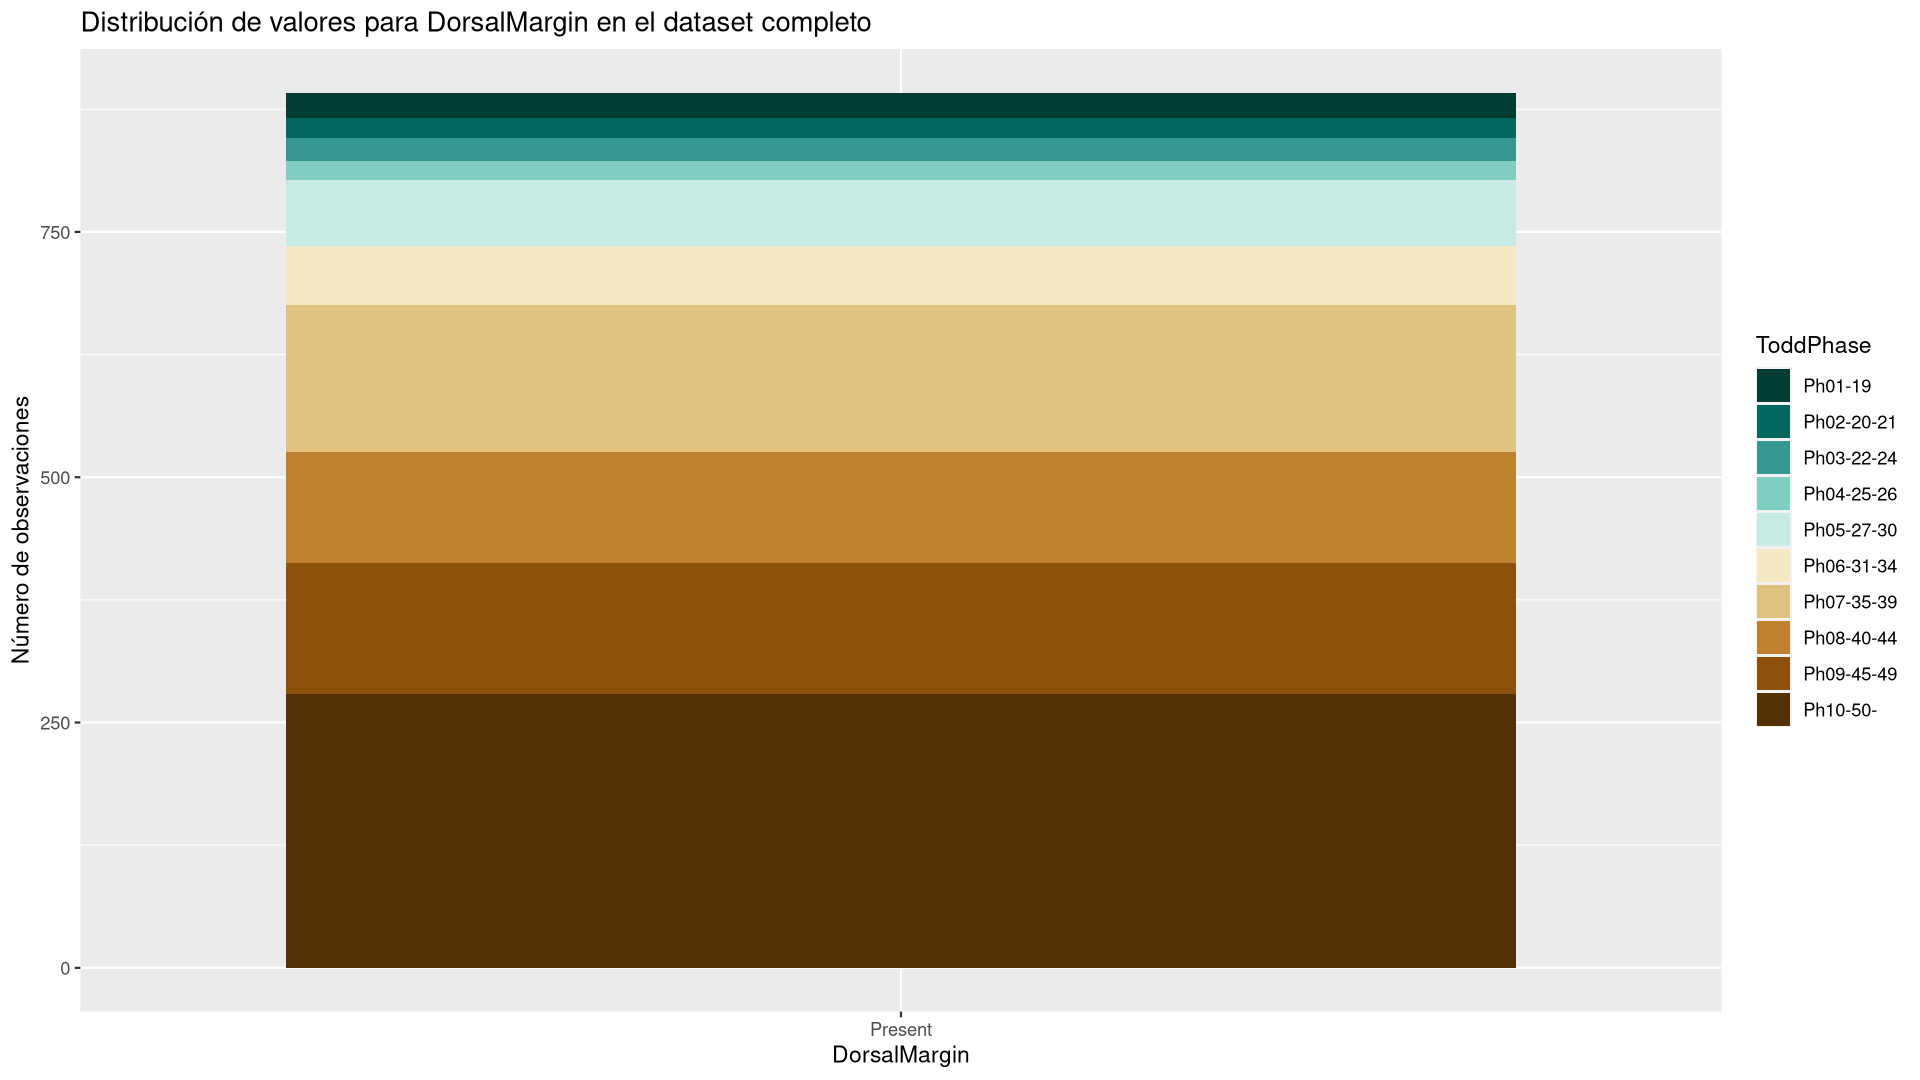
\includegraphics[width = \textwidth]{conjunto_datos/densidad_DorsalMargin_completo.png}
	\caption{Distribución de los valores de DorsalMargin en el conjunto de datos completo.}
	\label{fig:densidad_DorsalMargin_completo}
\end{figure}


En este caso \texttt{DorsalMargin} vemos como no aporta información alguna, ya que solo toma un valor independientemente de la fase de edad. En este caso podemos eliminar esta característica a la hora de entrenar el modelo ya que no aportaría información alguna al modelo, aunque los modelos que utilizaremos deberían ser capaces de inferir esto y no usar esta variable.


\begin{figure}[H]
	\centering
	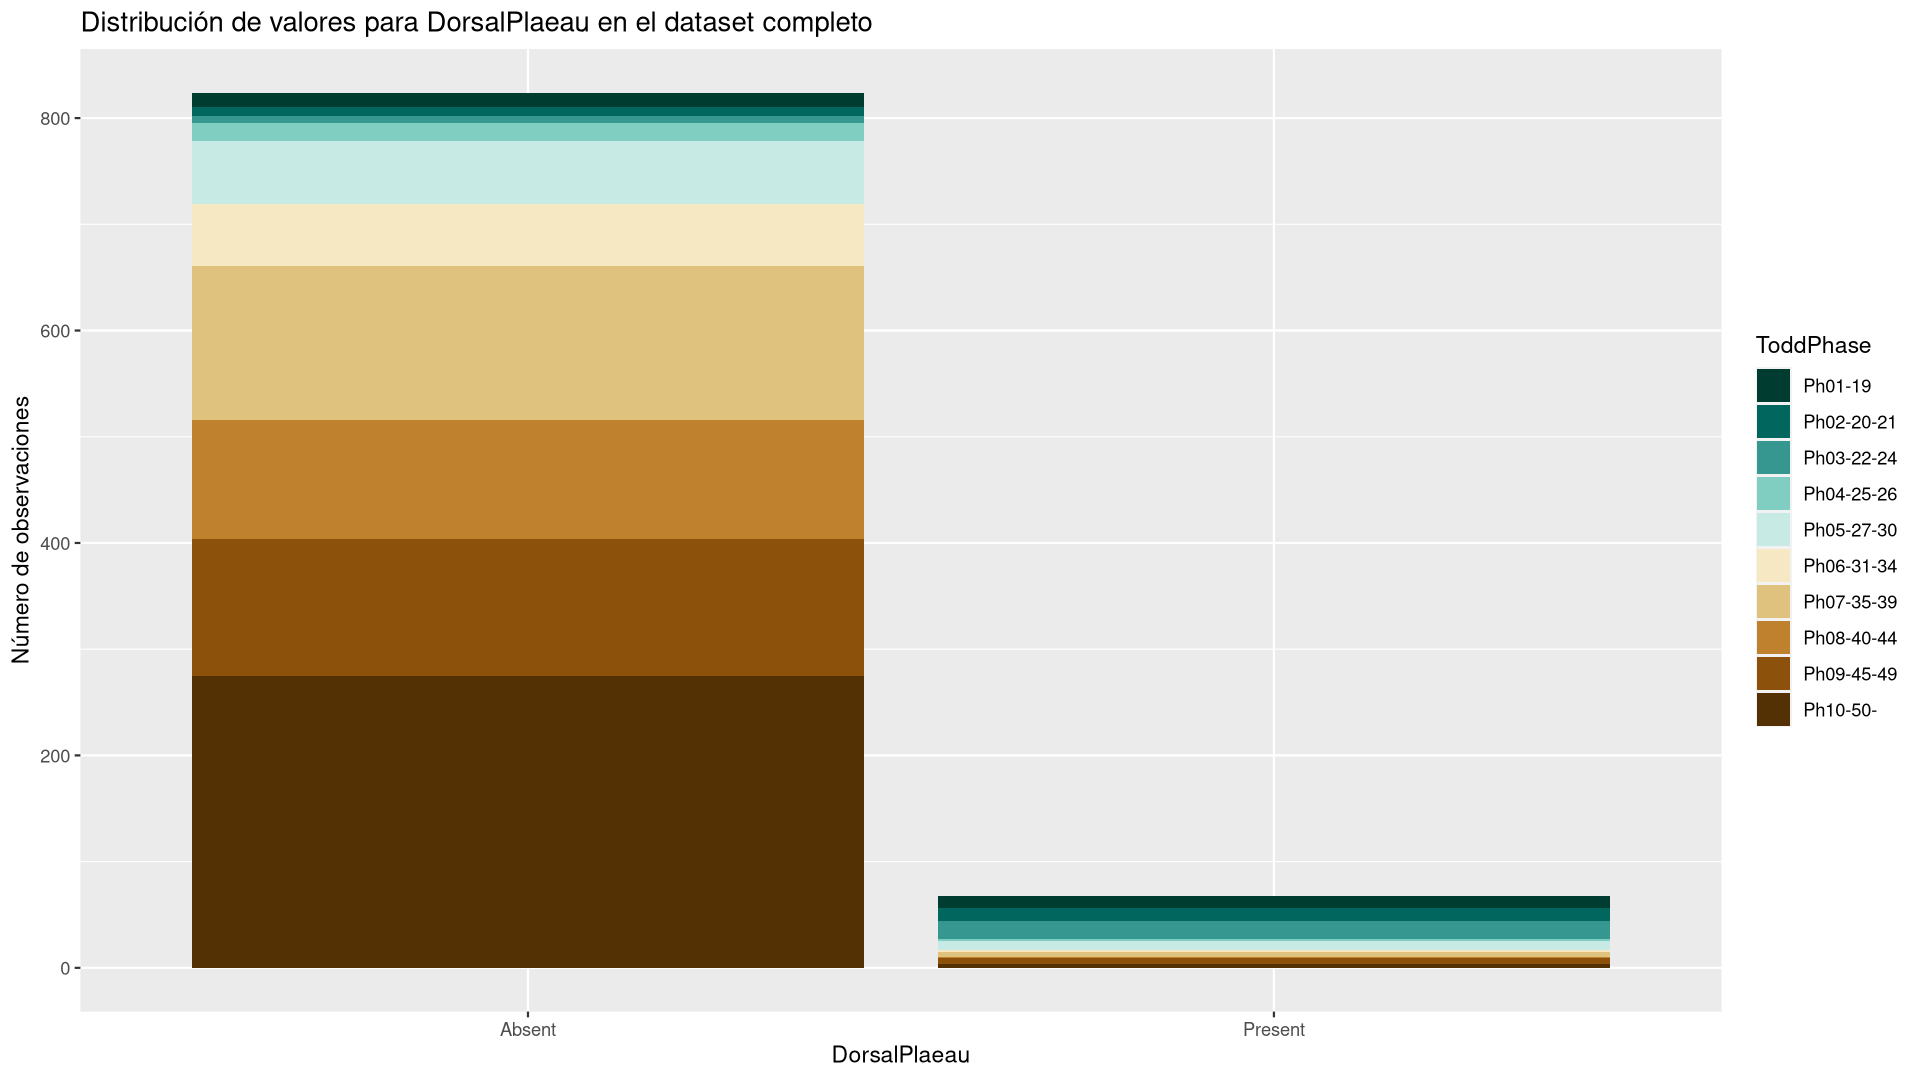
\includegraphics[width = \textwidth]{conjunto_datos/densidad_DorsalPlaeau_completo.png}
	\caption{Distribución de los valores de DorsalPlaeau en el conjunto de datos completo.}
	\label{fig:densidad_DorsalPlaeau_completo}
\end{figure}

Para los valores de \texttt{DorsalPlaeau} vemos como si que toma distintos valores, sin embargo estos no nos aportan mucha información, ya que tanto para \texttt{Absent} como para \texttt{Present} contamos con observaciones de todo tipo de fases, tanto altas como bajas, luego a priori no podemos saber si este predictor será de gran utilidad.


\begin{figure}[H]
	\centering
	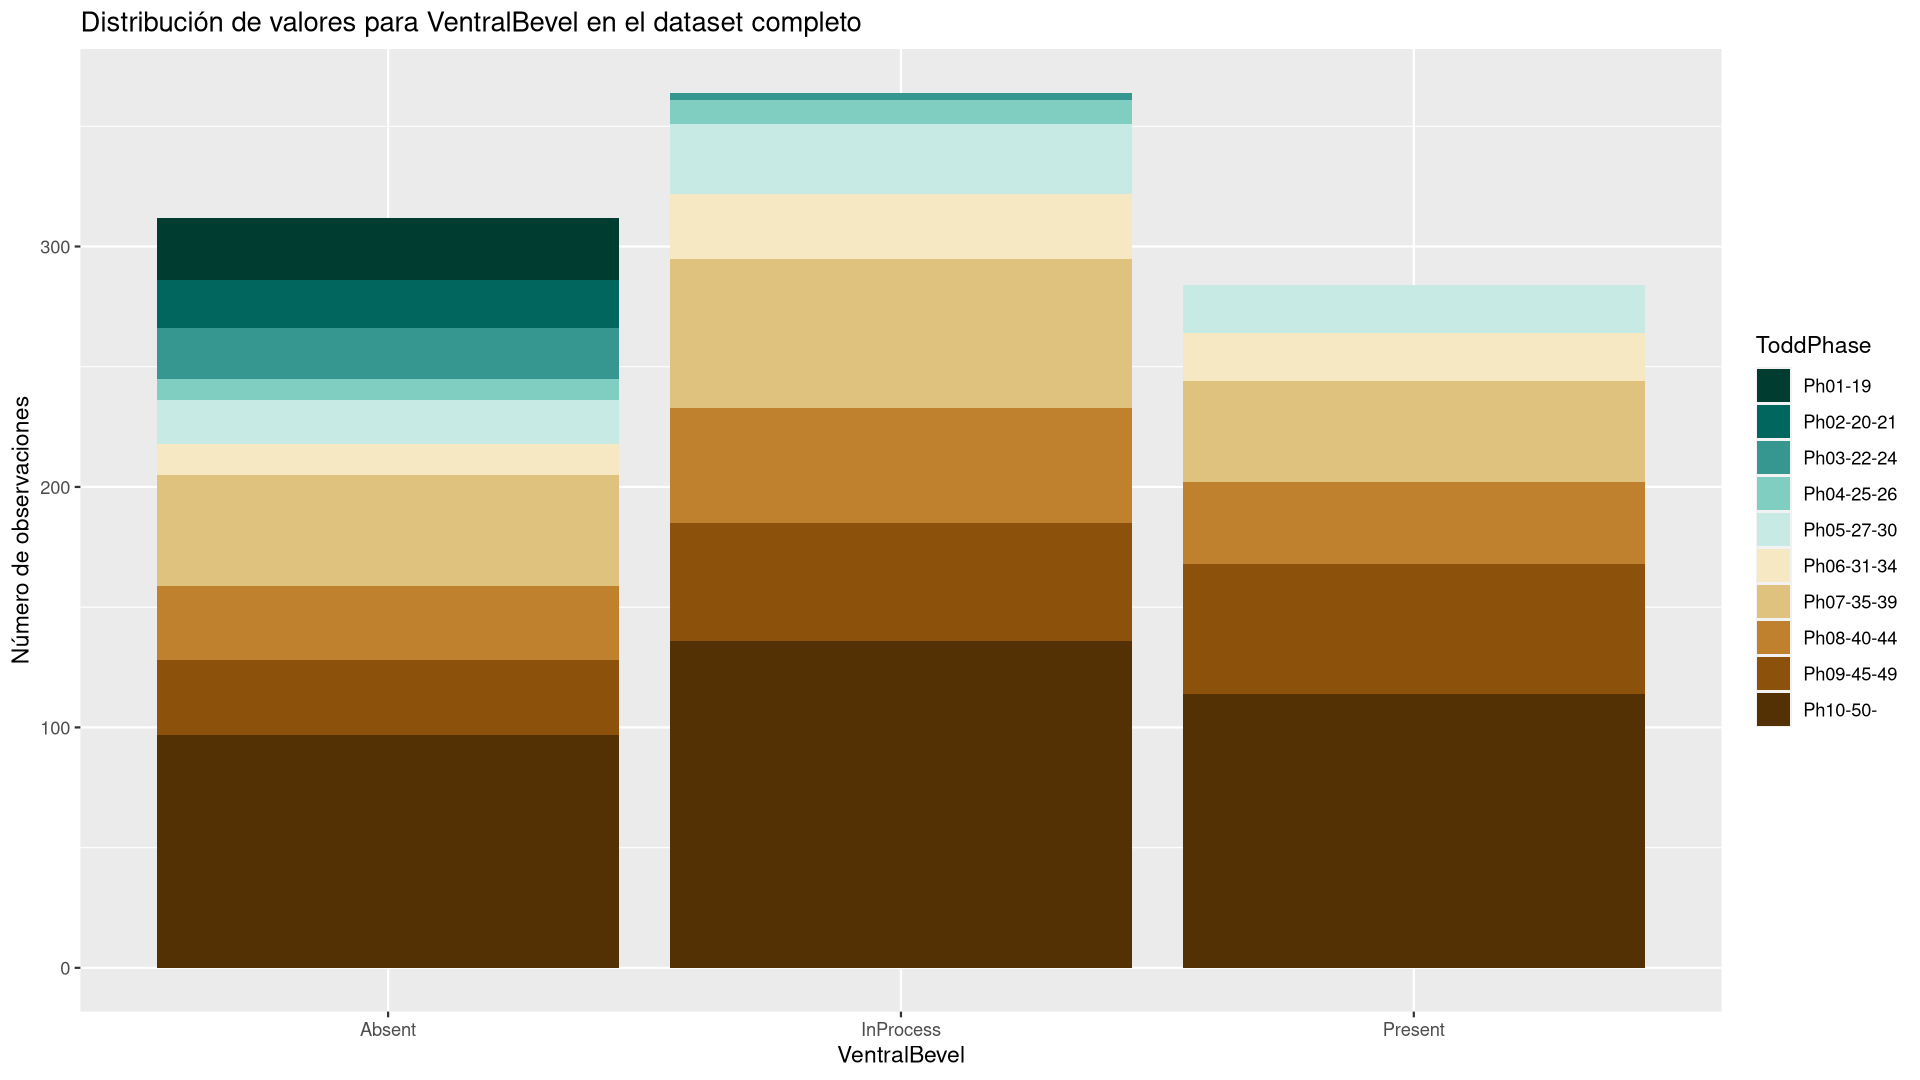
\includegraphics[width = \textwidth]{conjunto_datos/densidad_VentralBevel_completo.png}
	\caption{Distribución de los valores de VentralBevel en el conjunto de datos completo.}
	\label{fig:densidad_VentralBevel_completo}
\end{figure}

Aunque con \texttt{VentralBevel} vemos como para los distintos valores tenemos una gran variedad de clases, si que podemos sacar algunas conclusiones de este gráfico, voy a comentarlas según cada valor que puede tomar esta variable. Empezando con \texttt{Absent}, podemos ver como no podemos sacar ninguna conclusión, al tener observaciones de todo tipo de fases. Con \texttt{InProcess} se observa que aunque sigue existiendo observaciones de casi todas las fases, no tenemos de la fase uno, y las observaciones de la fase dos sin mínimas. Esto sumado a que con valores de \texttt{Present} solo se tienen observaciones de fases mayores a la fase cinco, este predictor nos puede ser de utilidad para acotar el resultado, ya que gran cantidad de observaciones toman el valor de \texttt{Present}, y con esto sabemos que son de una fase más alta y aunque siga existiendo variedad de clases, hemos conseguido acotarla.

\begin{figure}[H]
	\centering
	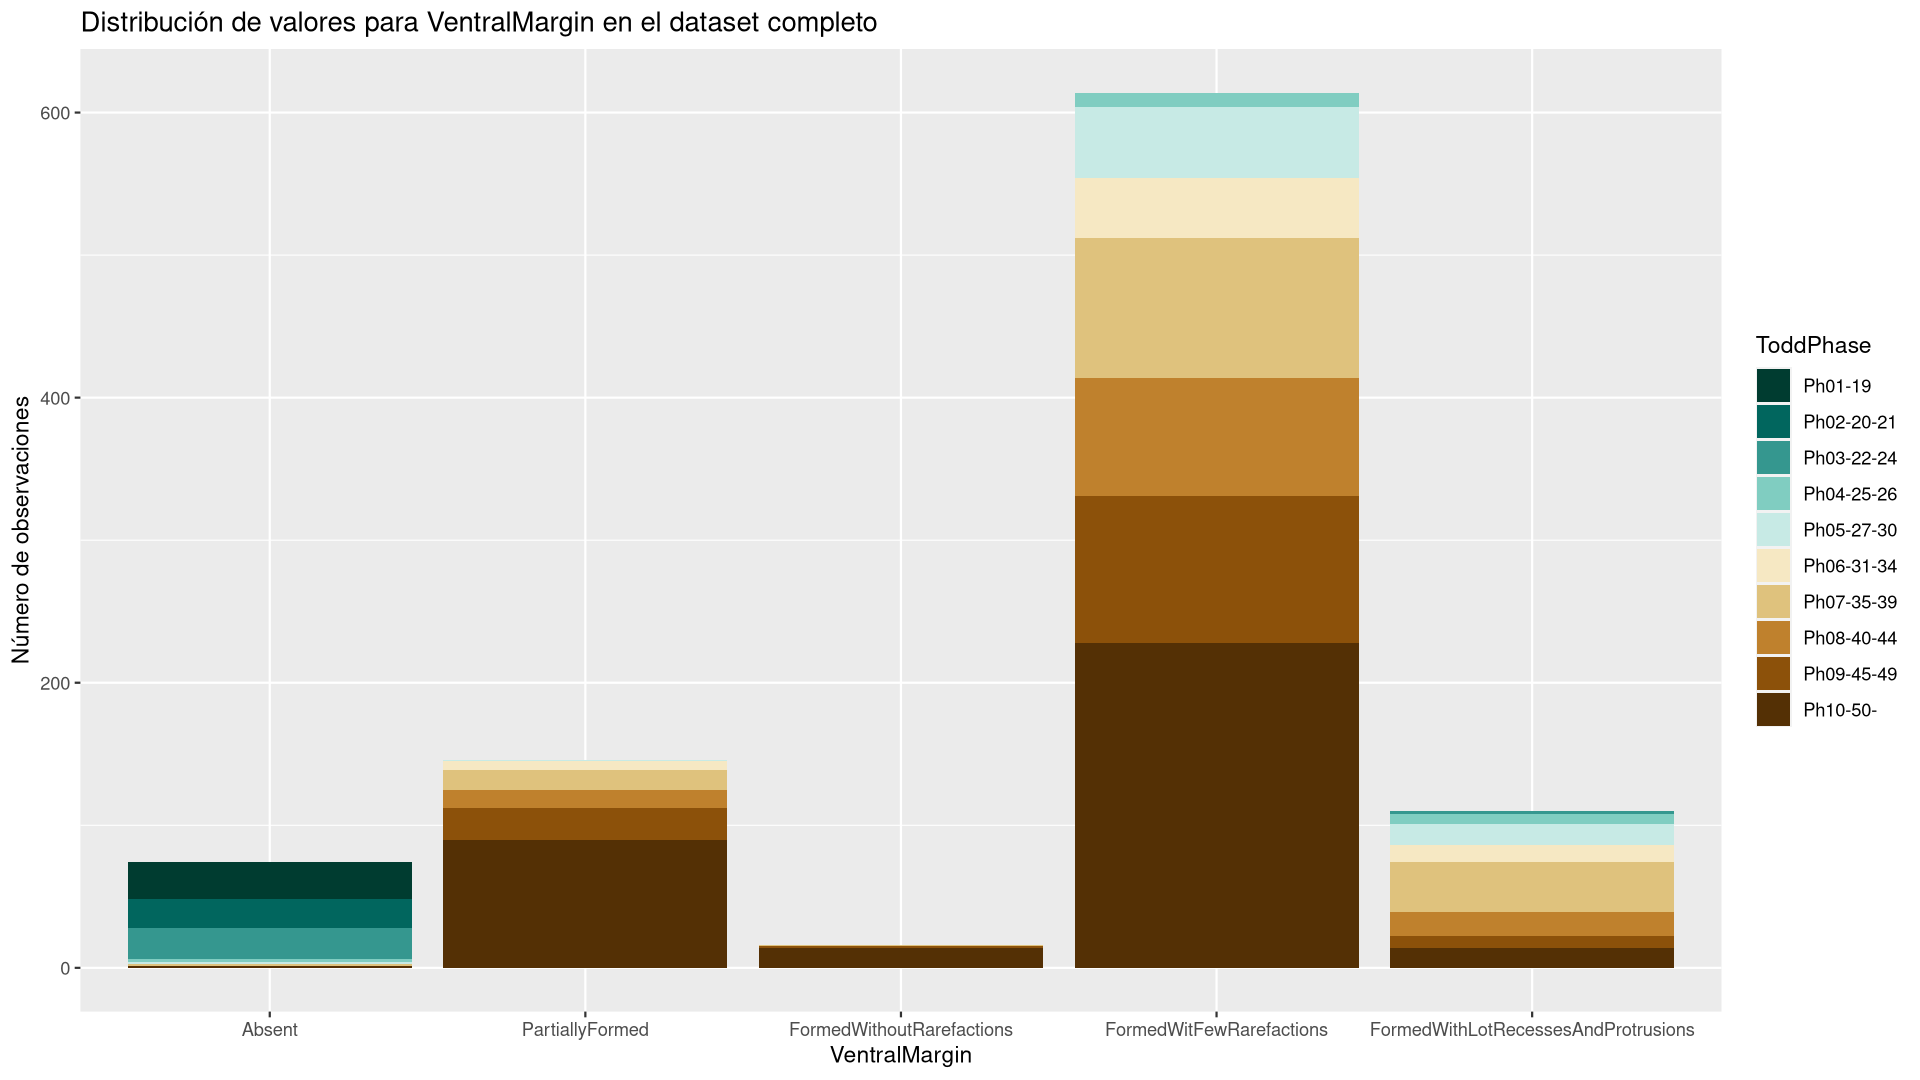
\includegraphics[width = \textwidth]{conjunto_datos/densidad_VentralMargin_completo.png}
	\caption{Distribución de los valores de VentralMargin en el conjunto de datos completo.}
	\label{fig:densidad_VentralMargin_completo}
\end{figure}


Para \texttt{VentralMargin} vemos como claramente si toma el valor de \texttt{Absent} nos indica que la observación de una fase temprana, si toma el valor de \texttt{PartiallyFormed} estamos ante una observación de una fase mayor o igual a la sexta, y si toma el valor de \texttt{FormedWithoutRarefactions} se trata de una observación de la última fase. Con respecto al resto de valores, \texttt{FormedWithFewRarefactions} sigue teniendo una cantidad alta de fases, pero nos puede dar la información de que la observación no es de las tres fases más tempranas, mientras que \texttt{FormedWithLotRecessesAndProtrusions} no nos da ninguna información de la clase debido al solape de fases que existen.

% TODO: actualizar toda la parte de sobremuestro, explicando SMOTE, borderline-SMOTE, ADASYN,
% comentar como funciona en nuestro conjunto de datos


\subsubsection{Conclusiones del análisis de datos}

Como breve resumen a este análisis de datos realizado, podemos ver como claramente este problema está desbalanceado y además es de una gran dificultad debido al gran solapamiento entre las clases, haciendo más difícil la clasificación.

También hemos podido observar distintas situaciones donde la decisión de la fase es más clara, acotando el tramo de decisión unicamente a dos o tres fases, sin embargo esto sucede con muy pocas observaciones del conjunto de datos. Hay que recordar que esto se ha hecho con un análisis univariante, es decir, observando por separado cada variable, el modelo que utilicemos tendrá a su disposición cualquier combinación de variables, con lo que se espera encontrar una mayor separabilidad entre las fases de cara a obtener un buen resultado en el problema.

Además, se ha observado que uno de los predictores, \texttt{DorsalMargin}, no aporta información al tomar únicamente un valor para todas las observaciones, independientemente de la clase, por lo que podríamos eliminar esta variable. En caso de no eliminarla, deberíamos observar que o bien no se utiliza en las reglas que obtengamos, o siempre que aparezca el valor utilizado será \texttt{Present}, que es el que siempre toma en el conjunto de datos.

Una vez realizado este análisis de datos, pasamos a las distintas técnicas de preprocesamiento que utilizaremos.


\subsection{Preprocesamiento} \label{sobremuestreo}

En esta sección se discutirá el preprocesamiento a aplicar a los datos de cara a entrenar el modelo, tanto las propias transformaciones que aplicaremos a los datos, como si es necesario aplicar técnicas más avanzadas como sobremuestreo y las algunas propuestas para aplicarlo.

\subsubsection{Transformación de los datos}

Con respecto a las transformaciones de los datos, todo el conjunto de datos está formado por características categóricas, lo que simplificará en gran cantidad tanto la formulación de las reglas como la interpretabilidad, ya que no tendremos que manejar valores reales para las características, en cuyo caso se podría haber propuesto un sistema de reglas difuso. Por este motivo en este caso no será necesario aplicar ninguna transformación a los datos.

Si es cierto que podemos hacer una pequeña selección de características, ya que como hemos visto en el análisis inicial, en concreto en la figura \ref{fig:densidad_DorsalMargin_completo}, la característica \texttt{DorsalMargin} la podemos eliminar del conjunto de datos al no aportar información relevante, al solo tomar un valor.

Tras esto, pasamos a las propuestas para balancear el número de instancias de cada clase.

\subsubsection{Separación en conjunto de entrenamiento y test}

Tras eliminar la característica que no aportaba información, se realizará una separación de los conjuntos de datos en conjuntos de entrenamiento y de test. Esto es importante de cara a la validación del algoritmo, ya que es necesario comprobar que la propuesta se comporta adecuadamente con datos con los que no ha entrenado, aunque dentro de la propia fase de entrenamiento apliquemos una validación cruzada que se explicará más adelante.

Es importante realizar este paso antes de aplicar las técnicas de sobremuestreo para solucionar el balanceo de clases, ya que el conjunto de test no puede contener datos sintéticos, ya que se trata de una prueba real del modelo, como si fueran datos reales que nos han llegado sin etiquetar.

En este caso se ha seleccionado de forma aleatoria uniforme un 80\% de las observaciones del conjunto de datos como datos de entrenamiento y el 20\% restante como datos de test para cada conjunto de datos. Sobre este 80\% de datos serán los datos a los que apliquemos el balanceo de clases, ya que con estos datos son con los que vamos a entrenar el modelo de cara a realizar las predicciones.

\newpage

\subsubsection{Sobremuestreo: Discusión sobre su importancia en este problema}

Ya hemos visto en el análisis de los datos la cantidad de observaciones con las que contamos de cada una de las clases del conjunto de datos \ref{fig:conteo_c}, y observamos como claramente de fases más tempranas apenas tenemos observaciones.

Los conjuntos de datos con esta distribución de observaciones son problemáticos, debido a que cualquier modelo que utilicemos tendrá un sesgo a favor de las clases mayoritarias a la hora de clasificar los datos. Esto se debe a que al realizar la clasificación, cuenta con tan pocos ejemplos de clases minoritarias que simplemente clasificando cualquier observación como de la clase mayoritaria es capaz de obtener un buen resultado de precisión.

Existen varias formas de corregir este problema, dependiendo del enfoque utilizado:

\begin{enumerate}
	\item Adaptando los datos: Se intentan conseguir más muestras de la clase minoritaria, ya sean creados de forma sintética o intentando obtener más información del problema. También se puede reducir el número de observaciones de la clase mayoritaria si contamos con suficientes ejemplos en la clase minoritaria.
	\item Adaptando los algoritmos: Para cada una de las clases se añade un peso de penalización al clasificar erróneamente una observación, de forma que se penaliza más equivocarse al clasificar erróneamente una observación de la clase minoritaria que si el modelo se equivoca en una observación de la clase mayoritaria. Esto en realidad es contrarrestar el sesgo inicial del modelo añadiendo un sesgo manual hacia las clases minoritarias.
\end{enumerate}

En nuestro caso, la primera solución será la que utilicemos debido a que de base el conjunto de datos es pequeño. Utilizaremos sobremuestro ya que no tenemos suficientes datos de las clases minoritarias como para realizar un submuestreo, y eso conllevaría una perdida de información demasiado grande.

% TODO: probar en el algoritmo añadir los pesos para corregir el sesgo
\newpage

\subsubsection{Sobremuestreo: Replicación aleatoria}

Una forma muy sencilla de aplicar sobremuestreo es replicar observaciones de las clases minoritarias de forma aleatoria, hasta llegar a tener un equilibrio entre las distintas clases.

Este método es muy simple, y puede tener ciertos problemas, ya que en realidad no ayuda a distinguir la frontera de decisión entre clases, simplemente evita que la penalización de ignorar una clase sea tan baja que el modelo pueda obviar dicha clase, sin embargo, una de las principales ventajas que tenemos con este método es que no estamos generando datos sintéticos, lo que podría conllevar a que el modelo entrenara con observaciones que no son realistas.

\subsubsection{Sobremuestreo: SMOTE}

SMOTE \cite{SMOTE} se trata de un método para conseguir balancear el número de datos para un problema de clasificación creando nuevos datos de las clases minoritarias de forma sintética. Fue propuesto en 2002 por varios investigadores de la Universidad de Florida del sur y la Universidad de Notre Dame.

Su funcionamiento se basa en tomar la clase minoritaria como clase positiva, y para cada elemento de dicha clase positiva buscar los $k$ vecinos más cercanos de la clase positiva. Una vez tenemos los $k$ elementos más cercanos, se crea un dato sintético entre cada vecino seleccionado y el punto original, escogiendo una zona del espacio al azar del segmento que une el vecino seleccionado y el punto original. De esta forma, modificando el número de vecinos a seleccionar, $k$, podemos ajustar el número de nuevos datos sintéticos.

\begin{figure}[H]
	\centering
	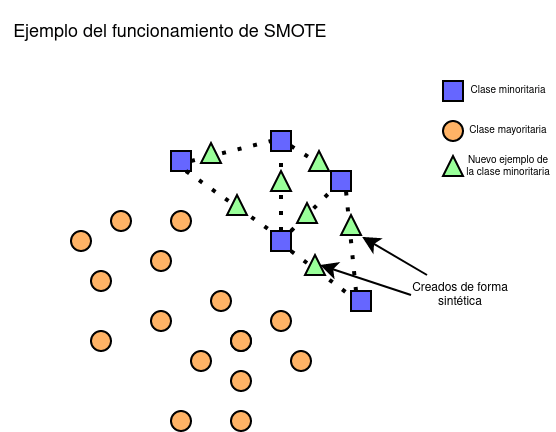
\includegraphics[scale = 0.6]{preprocesamiento/funcionamiento_smote.png}
	\caption{Ilustración de como funciona SMOTE.}
	\label{fig:funcionamiento_smote}
\end{figure}

\newpage

En su propuesta este método fue comparado con otros métodos de sobremuestreo:

\begin{figure}[H]
	\centering
	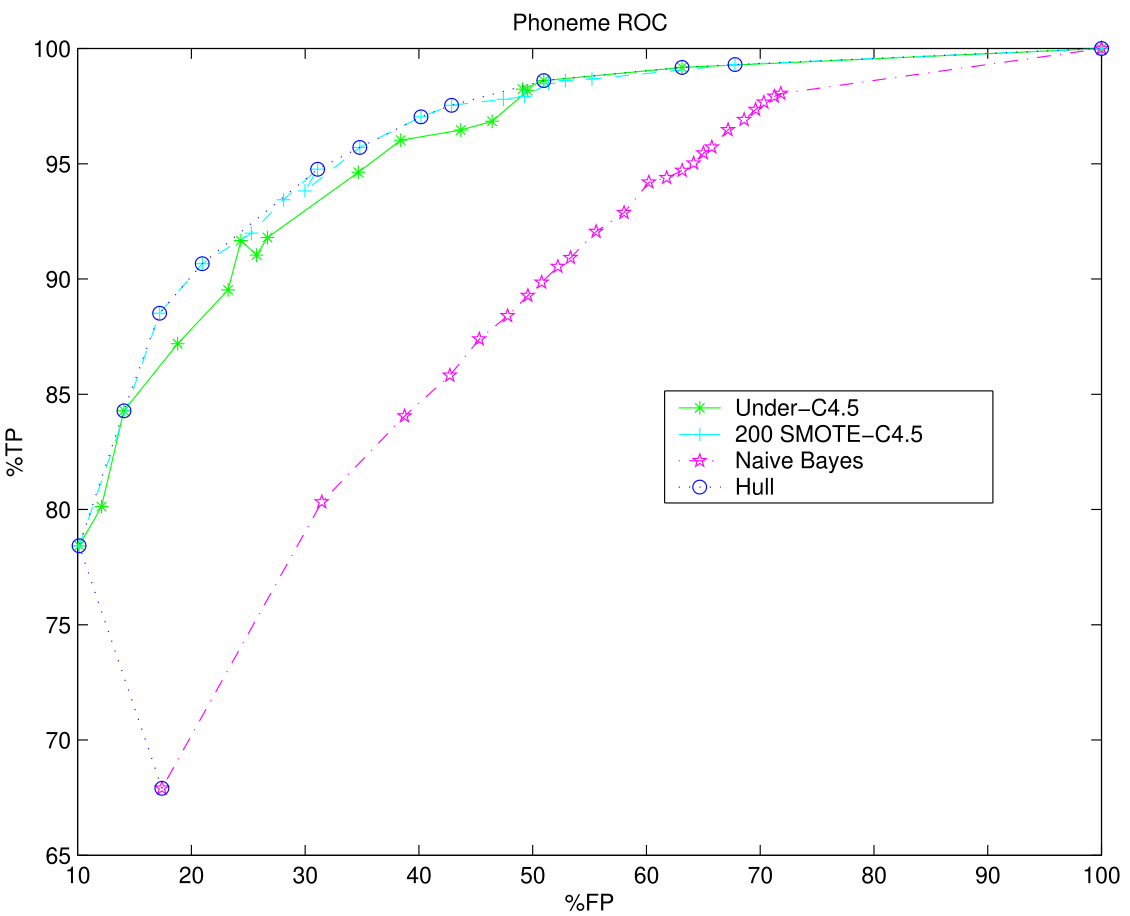
\includegraphics[scale = 1]{preprocesamiento/comparacion_ej_smote.png}
	\caption{Comparación de SMOTE con otros métodos de sobremuestreo en el conjunto de datos Phonome. En el eje X los falsos positivos y en el eje Y los verdaderos positivos. Imagen obtenida de \cite{SMOTE}.}
	\label{fig:comparacionSMOTE}
\end{figure}

Como vemos en la figura \ref{fig:comparacionSMOTE}, este método se comporta bastante bien en comparación con otros métodos y es capaz de obtener buenos resultados, sin embargo, tiene algunos problemas.

Uno de estos problemas es que cuando existe ruido entre las clases, o las clases se encuentran dispersas por el espacio de valores, gran parte de los valores sintéticos se encontrarán en una zona del espacio que no corresponde a su clase.

Este problema se hace mucho más presente en nuestro caso, al contar con tantas clases y con tantas características, y para resolverlo se propuso la variante Borderline-SMOTE.


\subsubsection{Sobremuestreo: Borderline SMOTE}

Borderline SMOTE \cite{BL-SMOTE} se trata de una variante de SMOTE que propone buscar los límites en el espacio de valores de la clase a obtener nuevos datos sintéticos, de forma que cuando se generen dichos datos nuevos, estén dentro de dichos límites. De esta forma evitamos problemas con conjuntos de datos con mucho ruido y múltiples clases.

En su artículo proponen dos variantes, una donde las nuevas muestras sintéticas son creadas a partir de todo el conjunto de datos, y otra donde las nuevas muestras solo se generan a partir de los datos considerados en el límite.


\begin{figure}[H]
    \centering
    \begin{subfigure}[b]{0.33\textwidth}
		  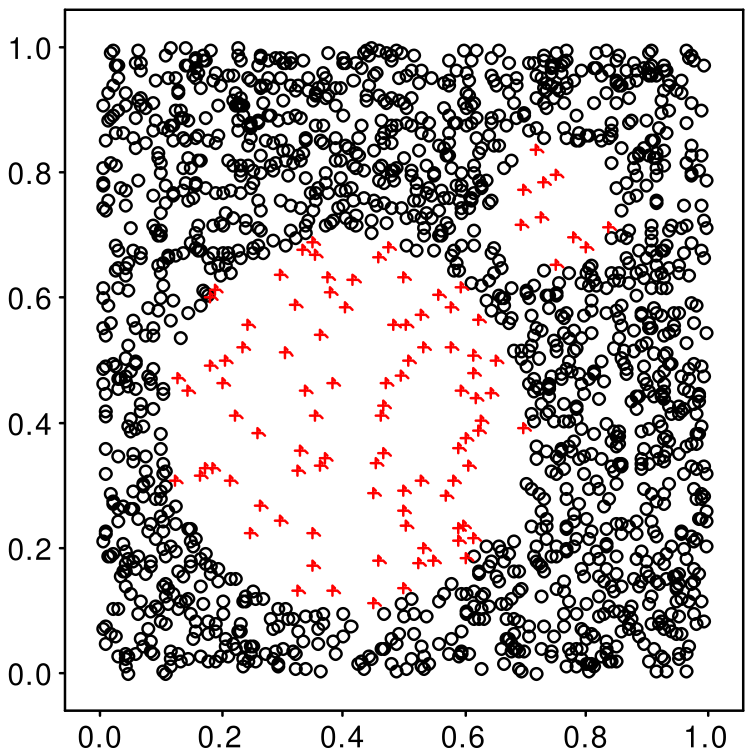
\includegraphics[width=\textwidth]{preprocesamiento/bl-smote-original.png}
        \caption{}
        \label{fig:blSMOTE-orig}
    \end{subfigure}
    \begin{subfigure}[b]{0.33\textwidth}
        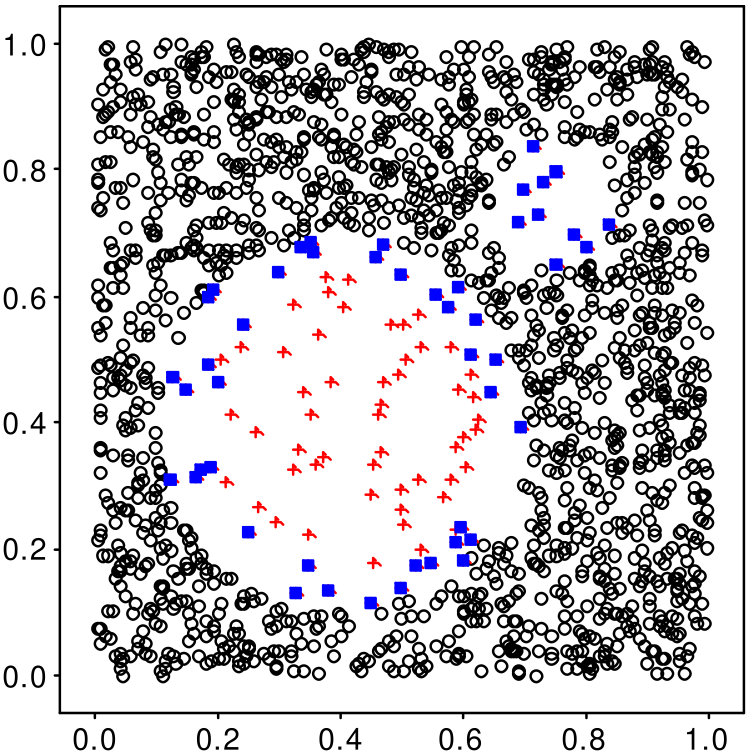
\includegraphics[width=\textwidth]{preprocesamiento/bl-smote-datos-borderline.png}
        \caption{}
        \label{fig:blSMOTE-border}
    \end{subfigure}
    \begin{subfigure}[b]{0.33\textwidth}
        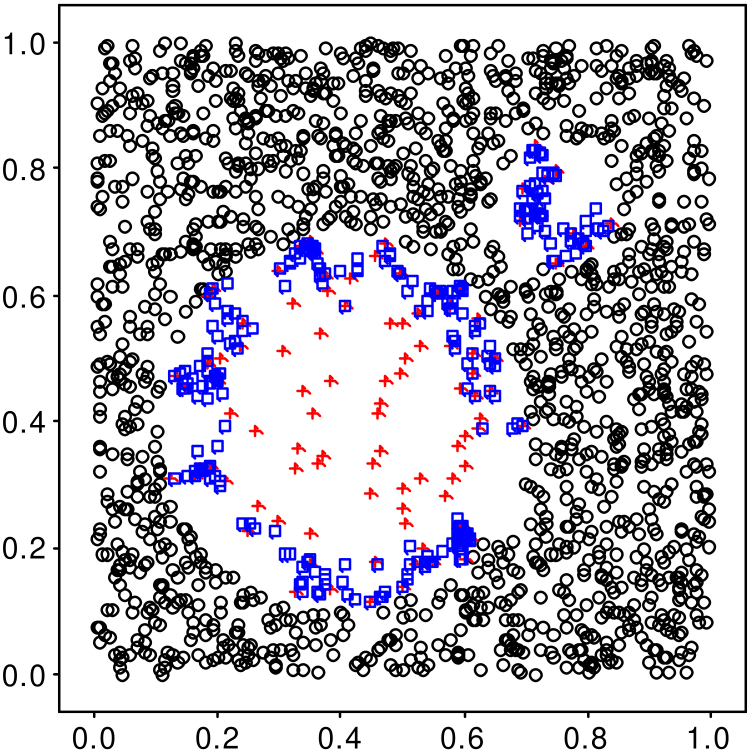
\includegraphics[width=\textwidth]{preprocesamiento/bl-smote-datos-sinteticos.png}
        \caption{}
        \label{fig:blSMOTE-sintetico}
    \end{subfigure}

    \caption{\ref{fig:blSMOTE-orig} Conjunto de datos original. \ref{fig:blSMOTE-border} datos que conforman el límite de la clase minoritaria (cuadros azules rellenos). \ref{fig:blSMOTE-sintetico} Nuevos datos generados de forma sintética dentro de los límites de la clase (cuadros azules no rellenos). Imagen obtenida de \cite{BL-SMOTE}.}
	 \label{fig:ejemploBL-SMOTE}

\end{figure}

Este método funciona de la misma forma que SMOTE a la hora de generar a los nuevos datos sintéticos, sin embargo, lo que hace es en lugar de utilizar todos los datos de la clase minoritaria, hace una preselección de datos, evitando los datos que son considerados como ruido y los datos donde es indiferente crear nuevas observaciones ya que no afectan a la frontera de decisión, es decir, se trata de una zona donde está claro que la clase es minoritaria. Esto hace que los puntos escogidos estén en la zona donde nos interesa tener datos, las fronteras entre las distintas clases, de forma que sea más facil diferenciar una clase de otra. Todo este proceso se ve ilustrado en figura \ref{fig:ejemploBL-SMOTE}.


Para comparar de forma gráfica SMOTE y BorderlineSMOTE podemos observar la siguiente ilustración utilizando datos generados de forma aleatoria con dos dimensiones:

\begin{figure}[H]
    \centering
	 \begin{subfigure}[b]{\textwidth}
		 \centering
		 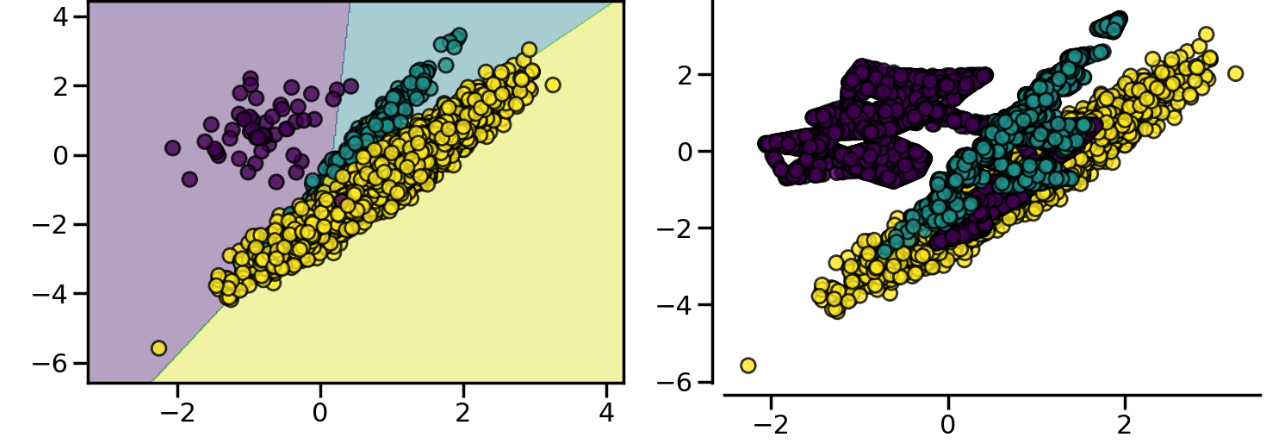
\includegraphics[width=0.8\textwidth]{preprocesamiento/resampling_smote.png}
		 \caption{A la izquierda bordes de las clases, y a la derecha sobremuestreo con SMOTE}
		 \label{fig:SMOTE-cmp}
	 \end{subfigure}

    \begin{subfigure}[b]{\textwidth}
		 \centering
		  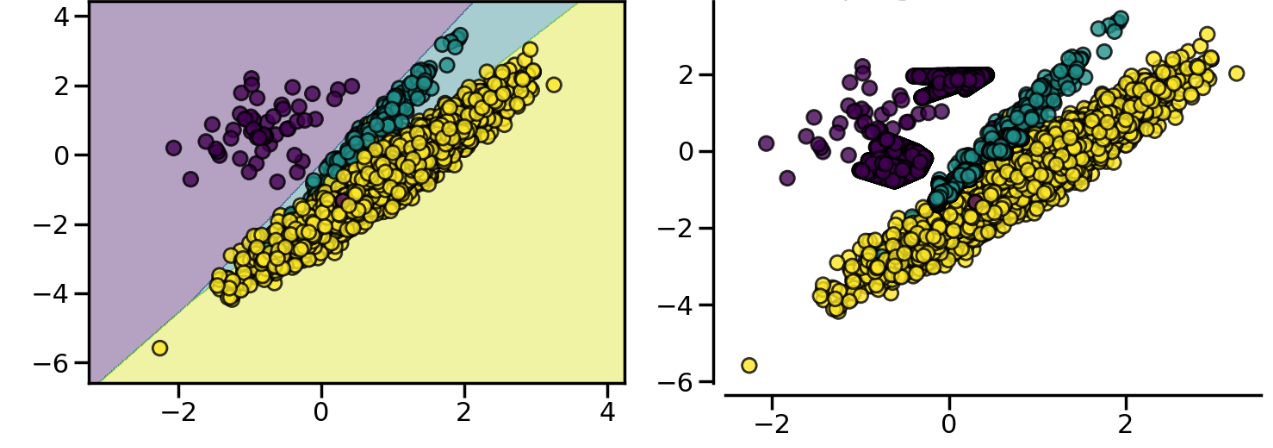
\includegraphics[width=0.8\textwidth]{preprocesamiento/resampling_blsmote.png}
        \caption{A la izquierda bordes de las clases, y a la derecha sobremuestreo con BorderlineSMOTE}
        \label{fig:BLSMOTE-cmp}
    \end{subfigure}

    \caption{Comparación de SMOTE y BorderlineSMOTE para un conjunto de datos generado aleatoriamente.}\label{fig:BLSMOTE-SMOTE}

\end{figure}

Esta claro que, como vemos en la figura \ref{fig:ejemploBL-SMOTE} y la figura \ref{fig:BLSMOTE-SMOTE}, esta técnica es mucho más versátil y conveniente que SMOTE.

\subsubsection{Sobremuestreo: Aplicación sobre datos categóricos}


Aplicar sobremuestreo aleatorio sobre cualquier tipo de dato es trivial, basta simplemente con replicar observaciones del conjunto de datos, sin embargo, cuando utilizamos propuestas más avanzadas podemos tener algunos problemas. Por ejemplo, la propuesta original de SMOTE utiliza el algoritmo k-NN para obtener los vecinos más cercanos, sin embargo, en nuestro caso tenemos un conjunto de datos donde todas las variables son categóricas, y por lo tanto no se puede realizar esta búsqueda de vecinos.

Para solucionar este problema utilizaremos la propuesta de SMOTE-N \cite{SMOTE}, también propuesta en el mismo trabajo donde se propuso SMOTE. Esta propuesta se basa en modificar el algoritmo k-NN utilizado en SMOTE por el k-NN propuesto por Stanfill y Waltz en 1986 \cite{kNNSMOTEN}, donde para aplicar el k-NN a un conjunto de datos categóricos utilizaban una versión modificada de la métrica de diferencia de valor, donde la distancia se basaba en el grado de diferencia entre los valores categóricos.

Por otro lado, BorderlineSMOTE no propone ninguna modificación para solucionar este problema, sin embargo como las características de nuestro conjunto de datos toman valores ordenados, como por ejemplo el nivel de porosidad, o el nivel de surcos presentes, se han codificado los datos de forma ordinal, transformando cada observación a un vector de enteros, asignando un entero a cada nivel de los valores que pueden tomar para cada una de sus características. Con esta modificación hemos podido aplicar BorderlineSMOTE y después deshacer la codificación para obtener los resultados del sobremuestreo con las etiquetas originales.

\subsection{Análisis de datos tras el preprocesado}

Como vimos en la sección de análisis del conjunto de datos, vamos a analizar los datos obtenidos por sobremuestreo aleatorio, SMOTE y Borderline SMOTE. Debido a la similitud entre ambas lateralidades, en esta ocasión solo comentaremos los efectos que podemos ver en el conjunto de datos completo. Este análisis nos servirá para observar si la aplicación de estas técnicas de sobremuestreo ha funcionado para equilibrar el número de clases, y si ha tenido algún efecto negativo que podamos ver utilizando la información de cada variable por separado, como añadir ruido o solape a las clases aplicar estas técnicas.

\subsubsection{Análisis del conjunto completo tras aplicar sobremuestro aleatorio}

El nuevo conjunto de datos completo, tras aplicar sobremuestreo aleatorio, cuenta con 2780 observaciones.

\begin{figure}[H]
	\centering
	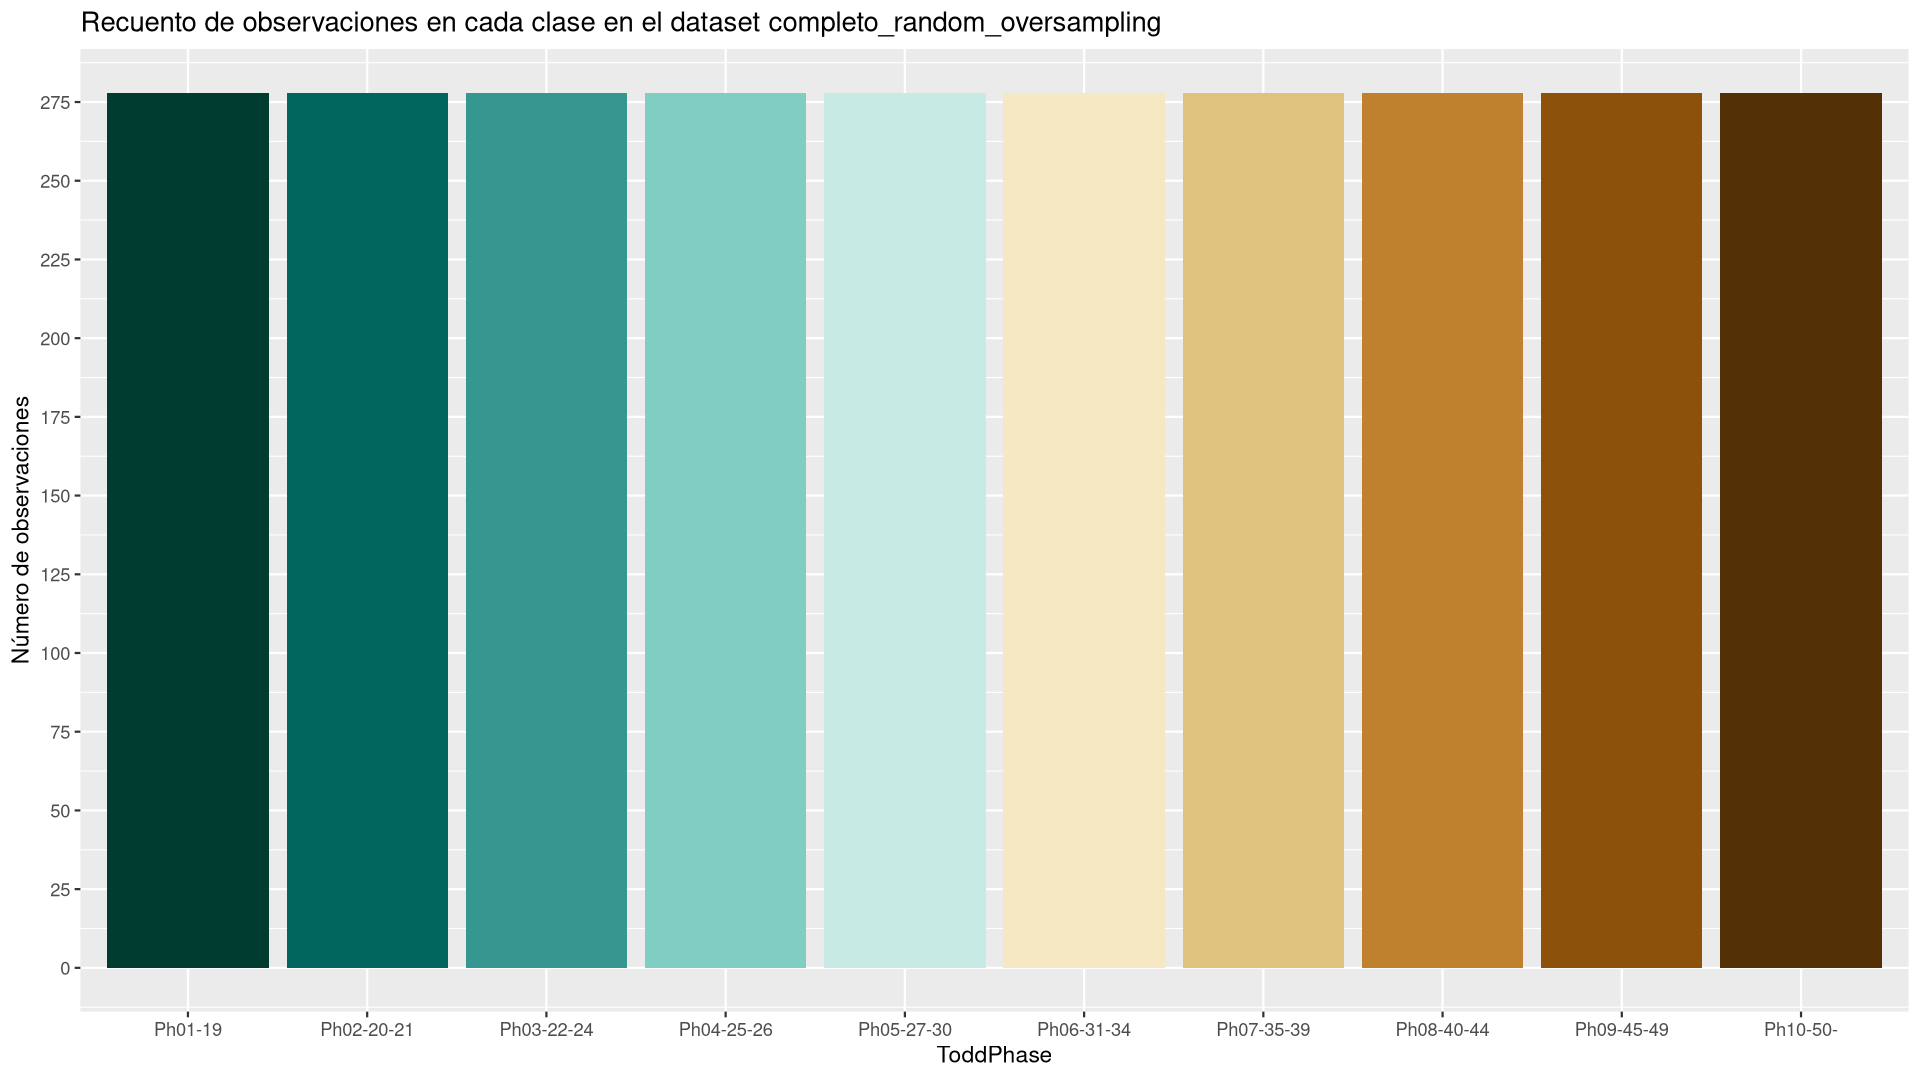
\includegraphics[width = \textwidth]{conjunto_random_oversampling/distribucion_clases_completo_random_oversampling.png}
	\caption{Número de datos por cada fase propuesta por Todd con el conjunto de datos completo tras aplicar sobremuestreo aleatorio.}
	\label{fig:conteo_c}
\end{figure}


Podemos ver que hemos solucionado el problema de balanceo de clases. En nuestro conjunto de entrenamiento todas las clases contarán con la misma cantidad de observaciones.

Debido a que este método lo único que ha hecho es replicar observaciones que ya teníamos, y no ha generado ningún dato sintético, podemos observar que si miramos en concreto cada característica simplemente vamos a ver que de cada clase existen más valores, pero manteniendo las diferencias y separaciones que veíamos antes en el análisis de datos con el conjunto original. Por ejemplo, al igual que en el conjunto de datos original, \texttt{IrregularPorosity} toma el valor \texttt{NotDefined} únicamente para fases bajas, es normal que esto ocurra ya que en realidad al replicar observaciones no estamos introduciendo ninguna nueva observación que pueda cambiar esto, por lo que todas las conclusiones sacadas anteriormente son las mismas para este caso.


\begin{figure}[H]
	\centering
	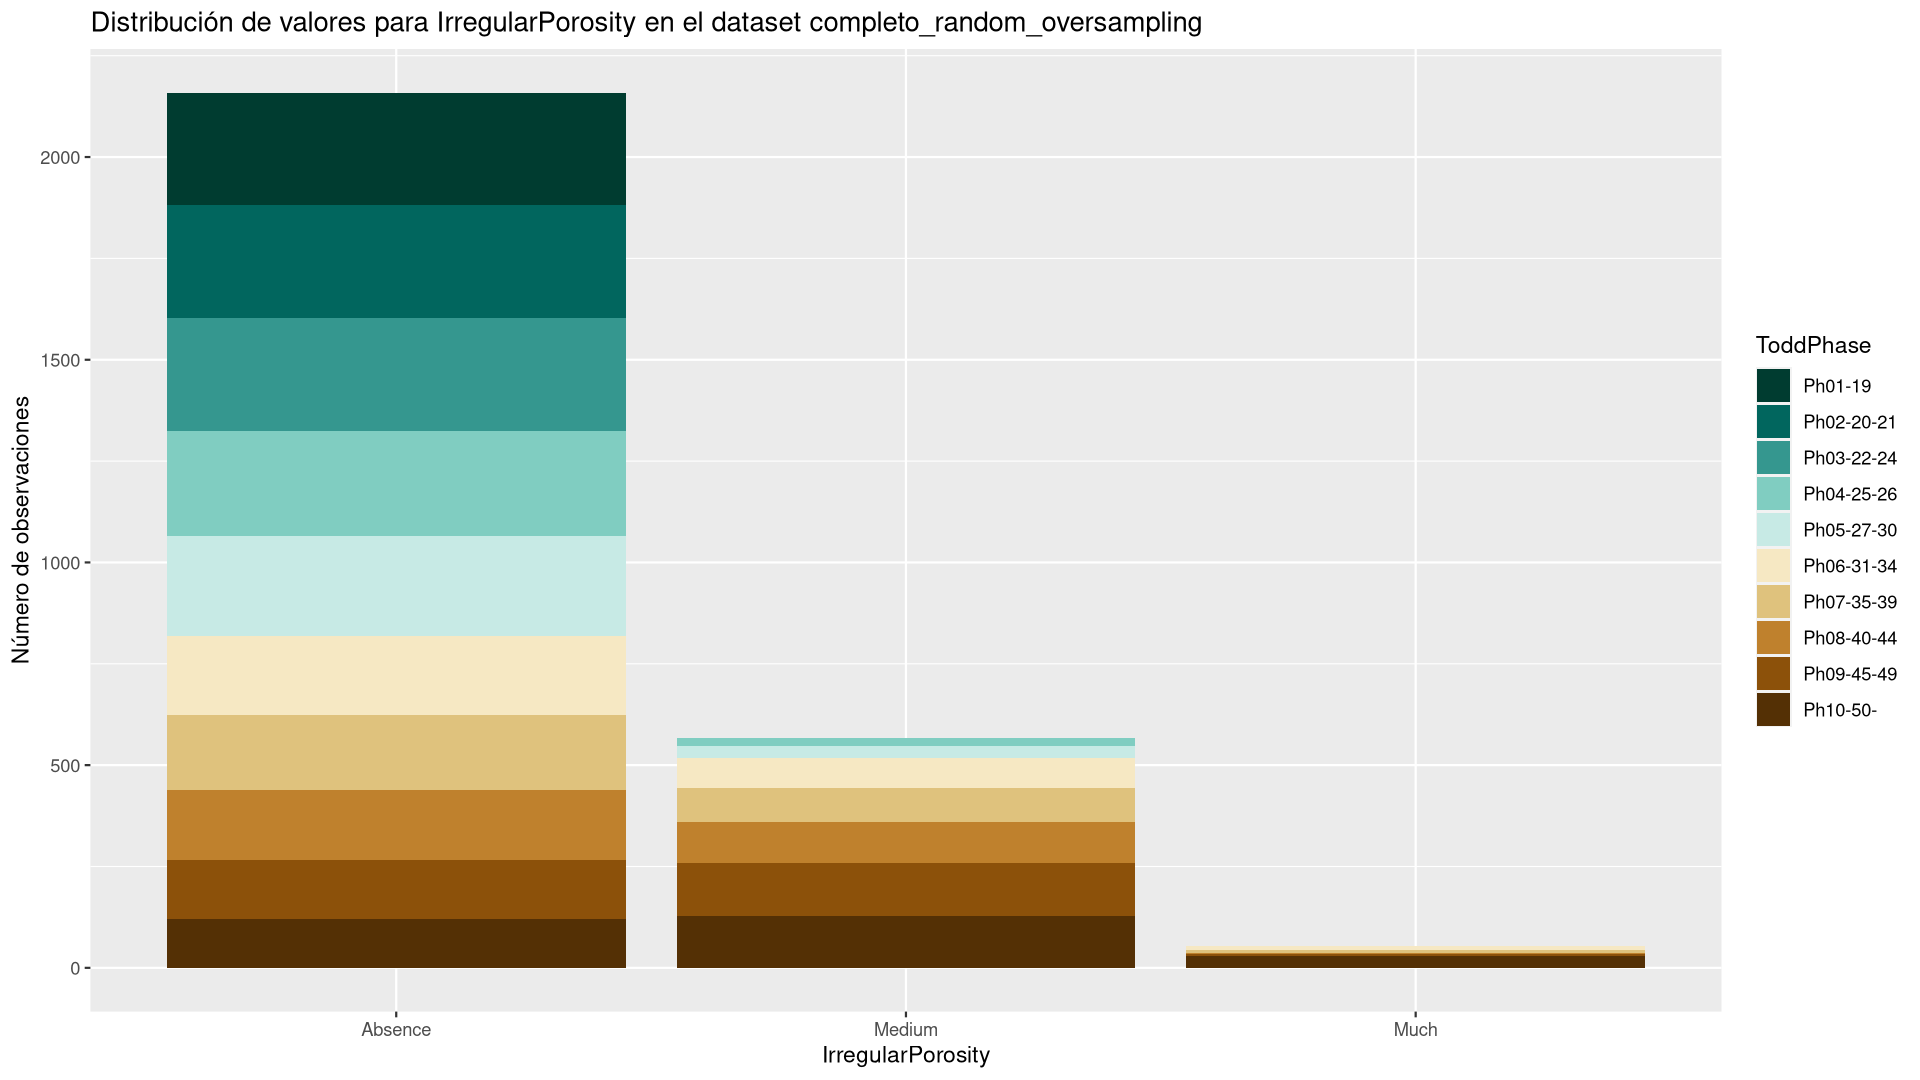
\includegraphics[width = \textwidth]{conjunto_random_oversampling/densidad_IrregularPorosity_completo_random_oversampling.png}
	\caption{Distribución de los valores de IrregularPorosity en el conjunto de datos completo tras aplicar sobremuestreo aleatorio.}
	\label{fig:densidad_IrregularPorosity_completo_random_oversampling}
\end{figure}




\begin{figure}[H]
	\centering
	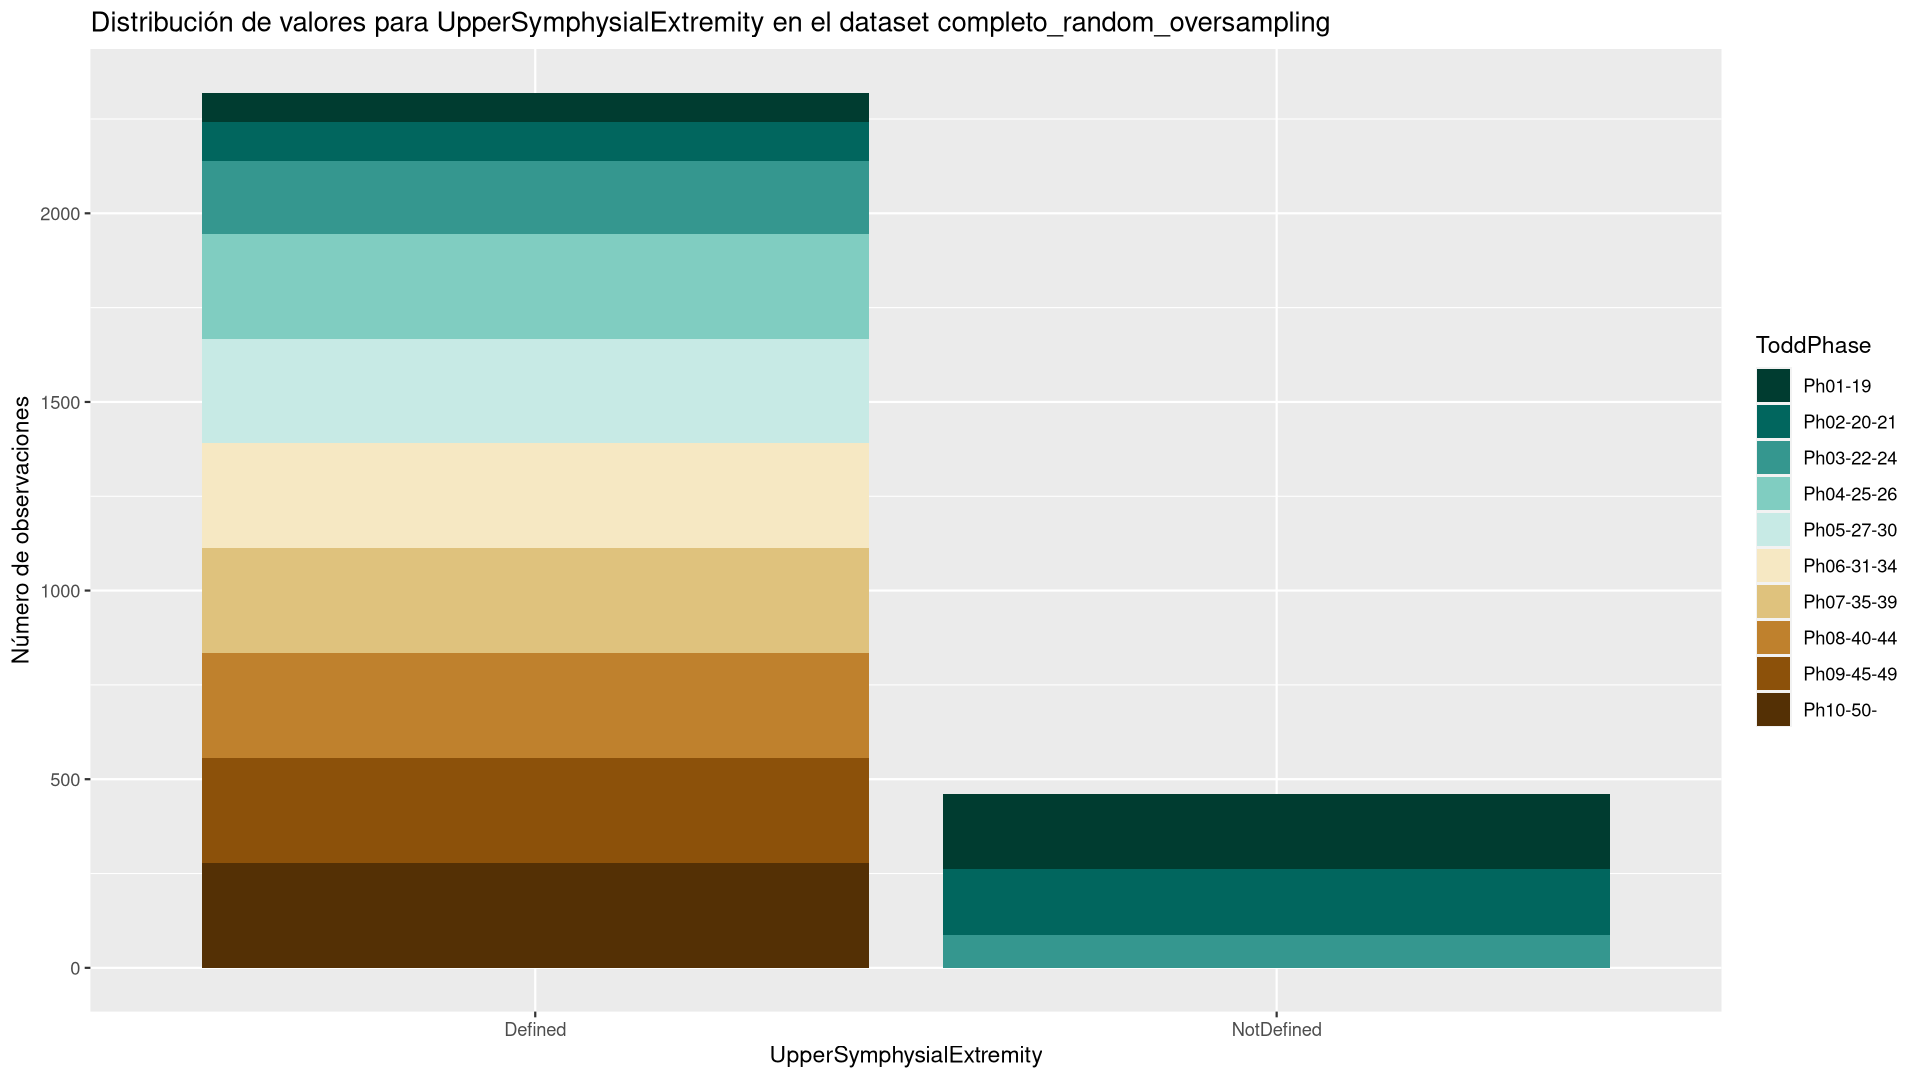
\includegraphics[width = \textwidth]{conjunto_random_oversampling/densidad_UpperSymphysialExtremity_completo_random_oversampling.png}
	\caption{Distribución de los valores de UpperSymphysialExtremity en el conjunto de datos completo tras aplicar sobremuestreo aleatorio.}
	\label{fig:densidad_UpperSymphysialExtremity_completo_random_oversampling}
\end{figure}


\begin{figure}[H]
	\centering
	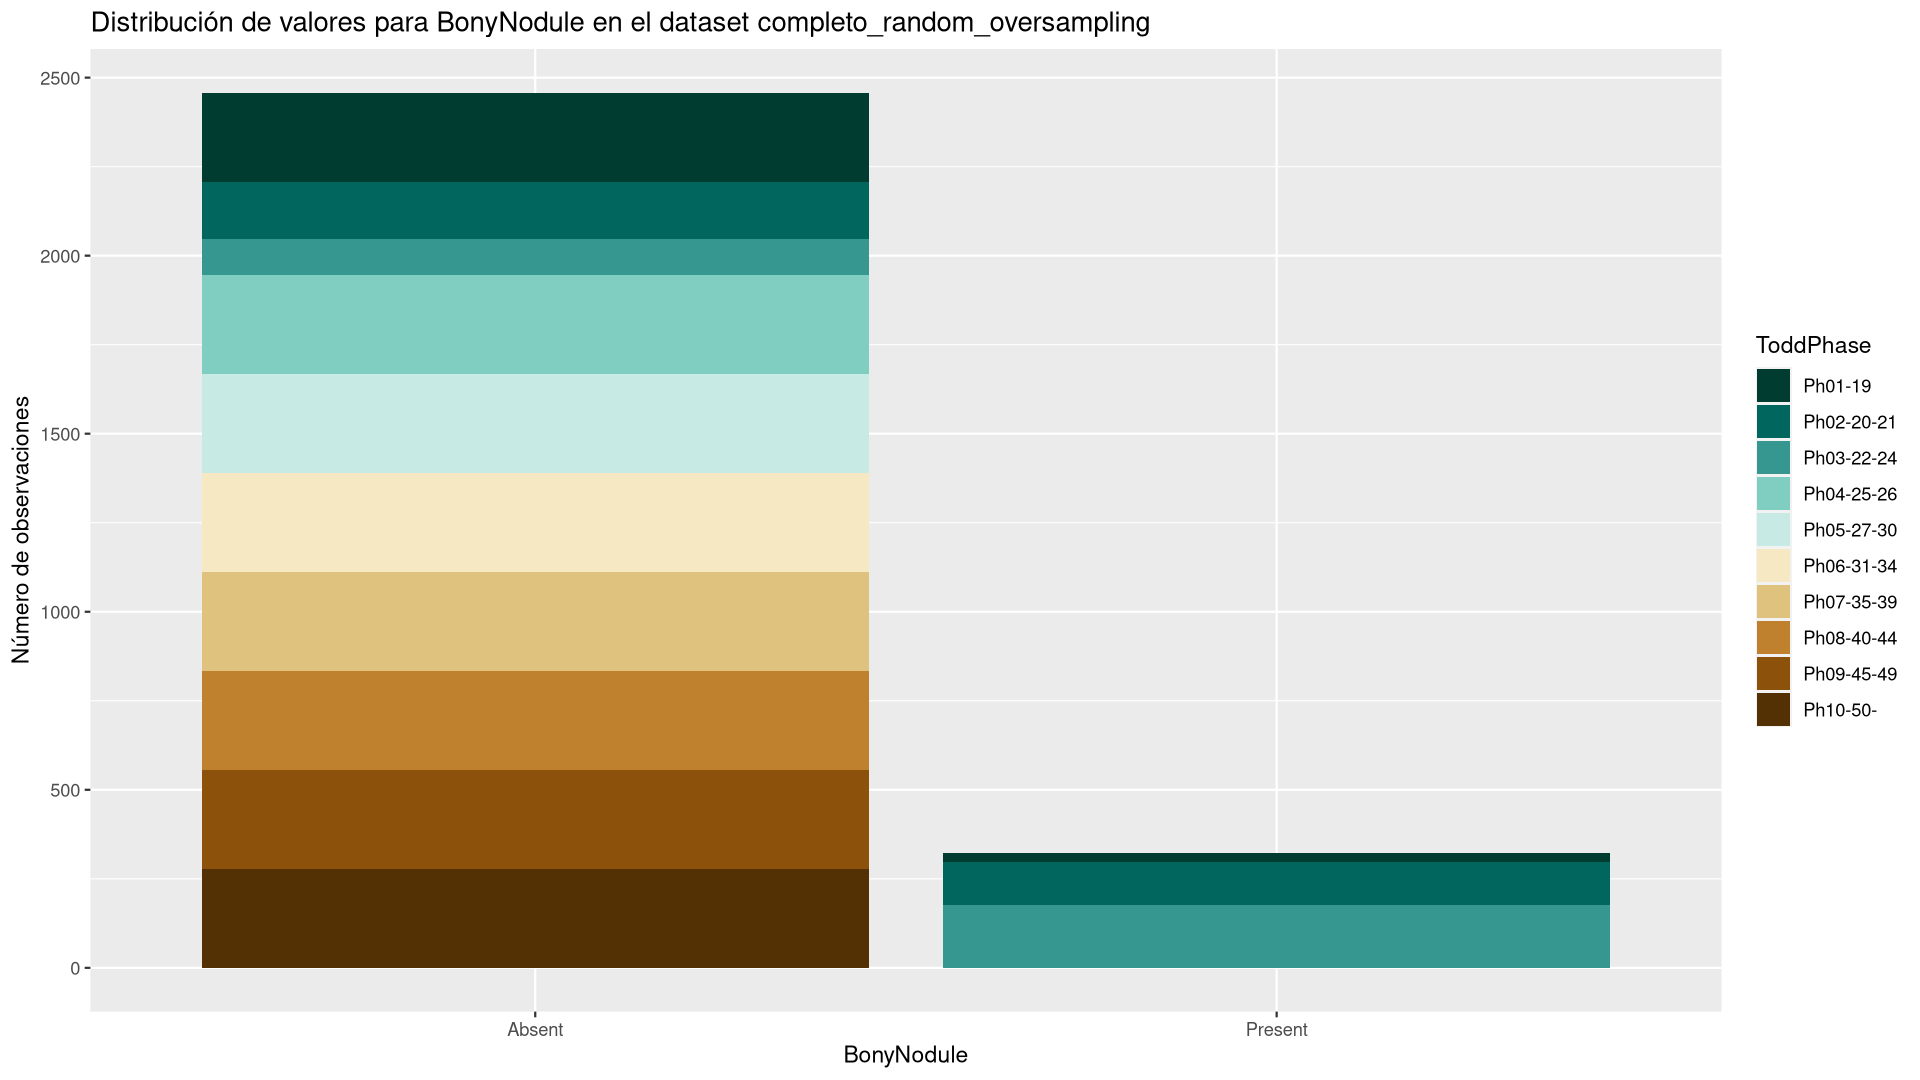
\includegraphics[width = \textwidth]{conjunto_random_oversampling/densidad_BonyNodule_completo_random_oversampling.png}
	\caption{Distribución de los valores de BonyNodule en el conjunto de datos completo tras aplicar sobremuestreo aleatorio.}
	\label{fig:densidad_BonyNodule_completo_random_oversampling}
\end{figure}



\begin{figure}[H]
	\centering
	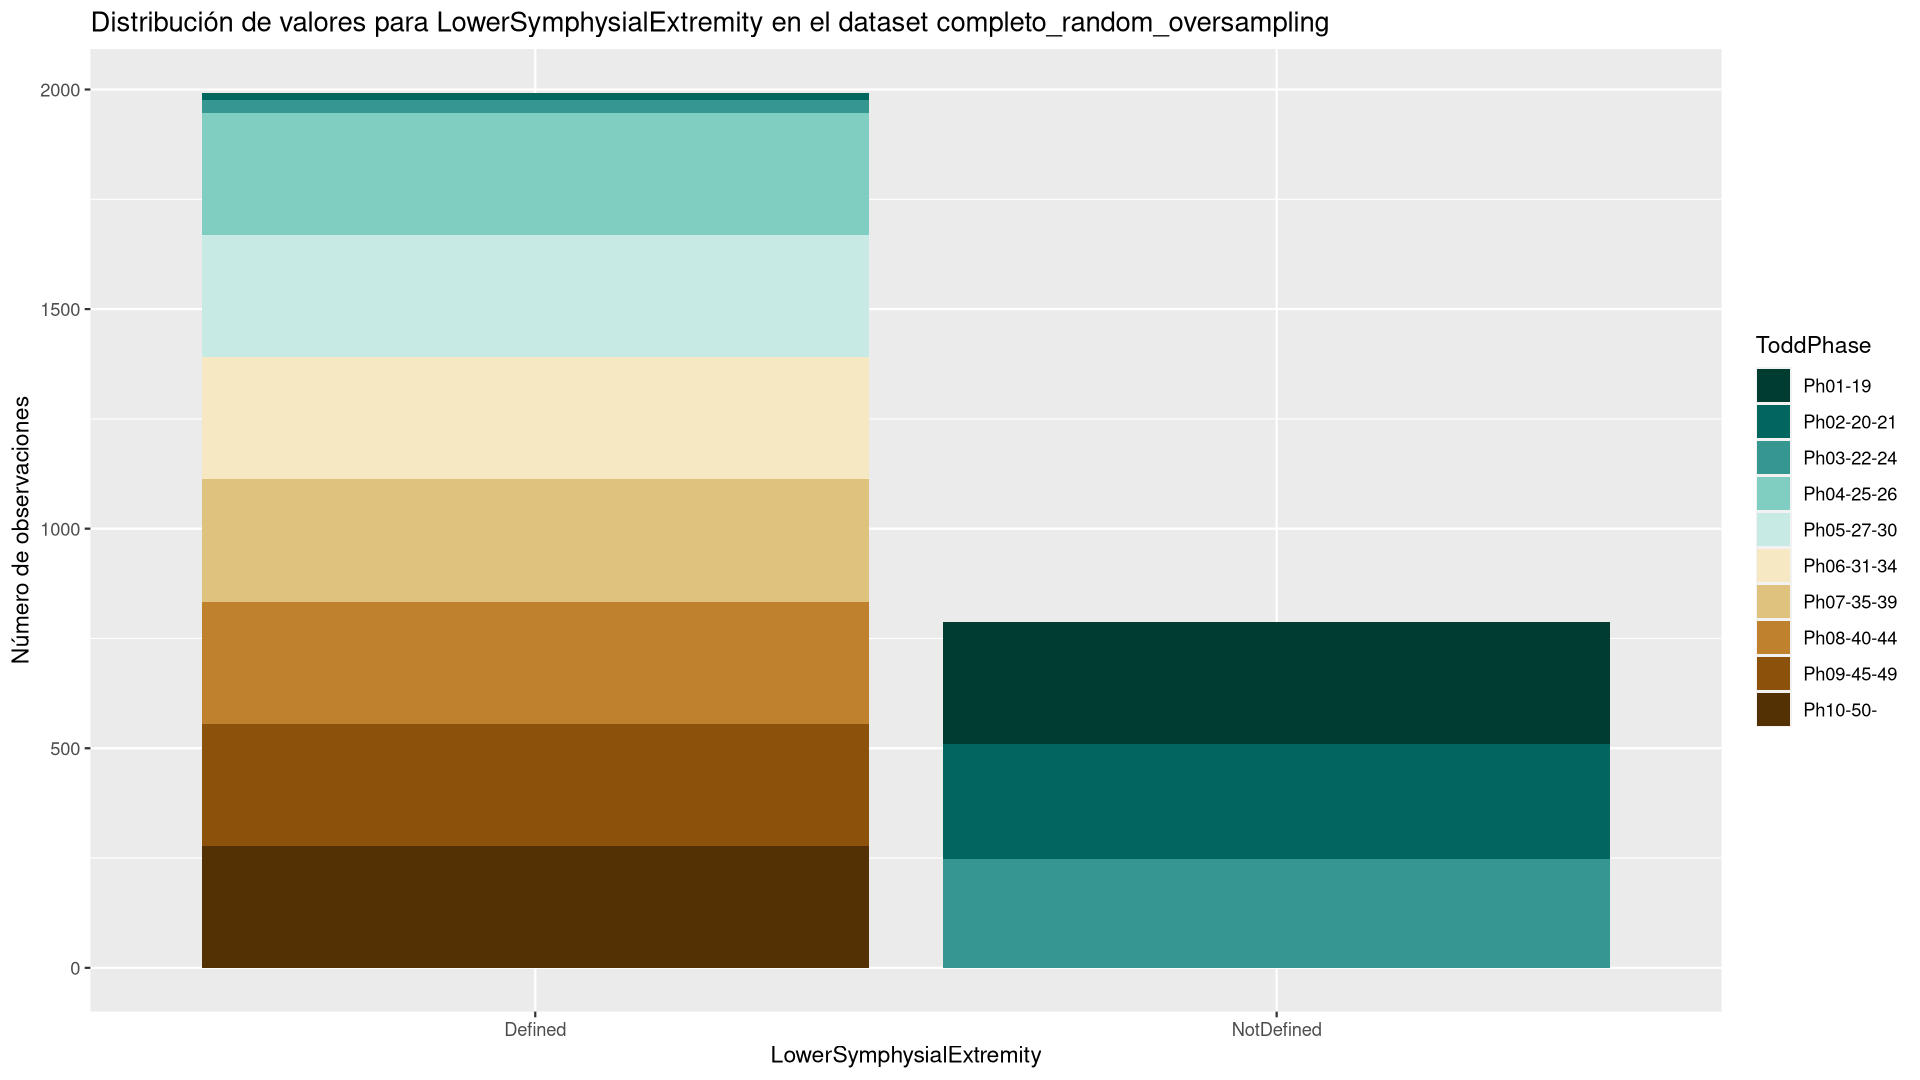
\includegraphics[width = \textwidth]{conjunto_random_oversampling/densidad_LowerSymphysialExtremity_completo_random_oversampling.png}
	\caption{Distribución de los valores de LowerSymphysialExtremity en el conjunto de datos completo tras aplicar sobremuestreo aleatorio.}
	\label{fig:densidad_LowerSymphysialExtremity_completo_random_oversampling}
\end{figure}


\begin{figure}[H]
	\centering
	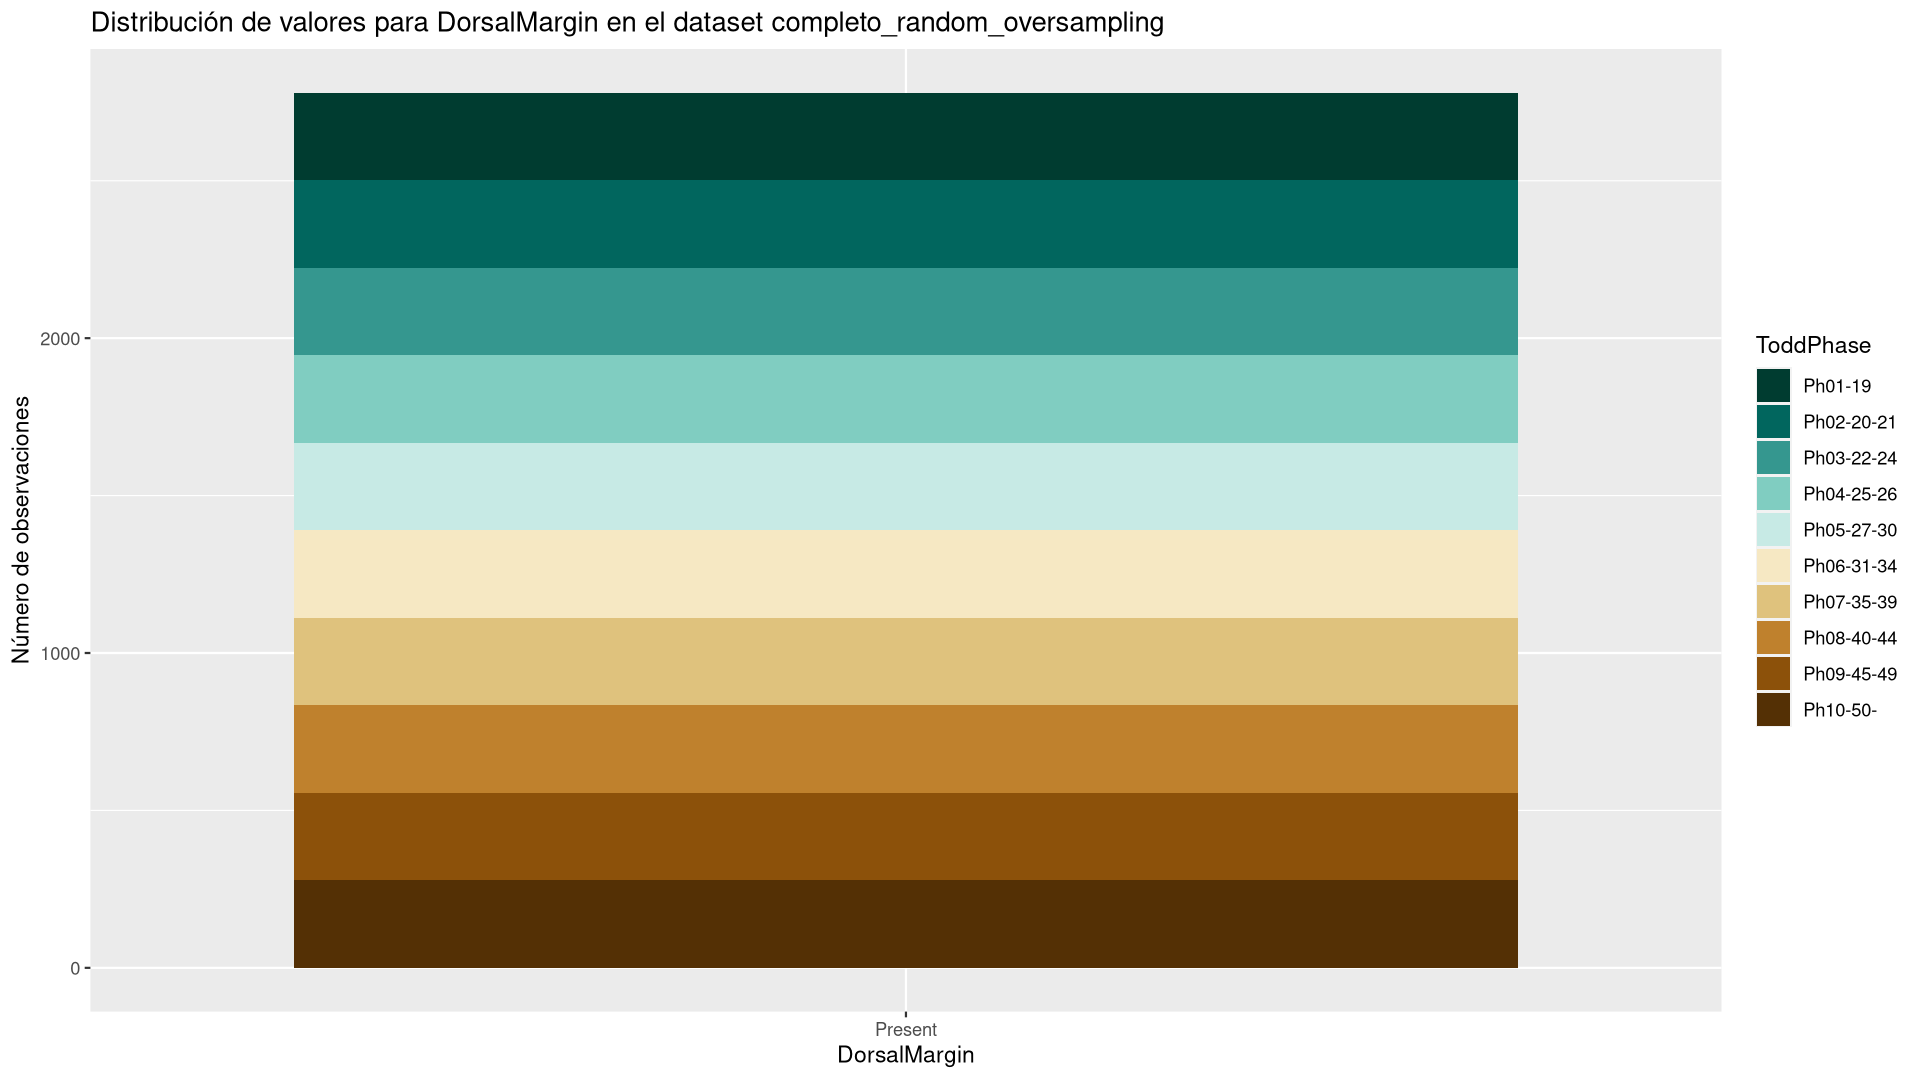
\includegraphics[width = \textwidth]{conjunto_random_oversampling/densidad_DorsalMargin_completo_random_oversampling.png}
	\caption{Distribución de los valores de DorsalMargin en el conjunto de datos completo tras aplicar sobremuestreo aleatorio.}
	\label{fig:densidad_DorsalMargin_completo_random_oversampling}
\end{figure}




\begin{figure}[H]
	\centering
	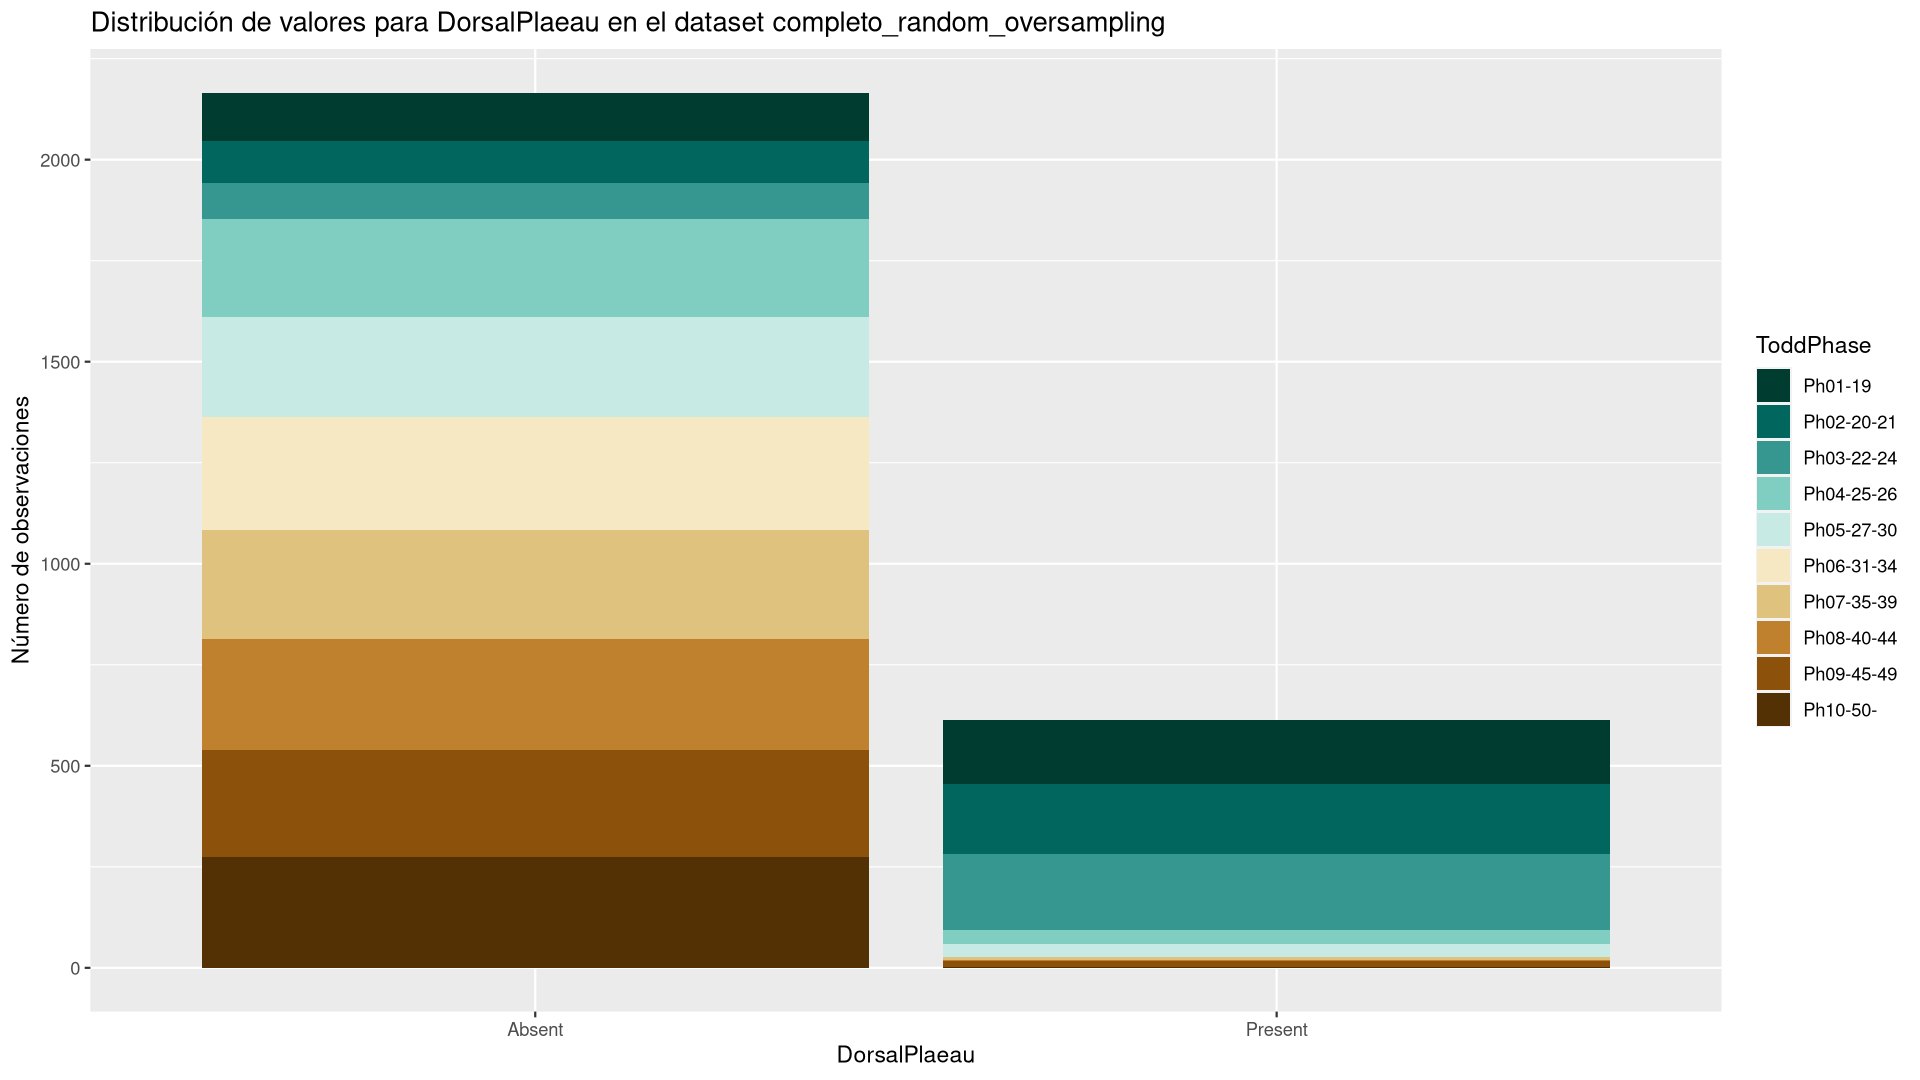
\includegraphics[width = \textwidth]{conjunto_random_oversampling/densidad_DorsalPlaeau_completo_random_oversampling.png}
	\caption{Distribución de los valores de DorsalPlaeau en el conjunto de datos completo tras aplicar sobremuestreo aleatorio.}
	\label{fig:densidad_DorsalPlaeau_completo_random_oversampling}
\end{figure}



\begin{figure}[H]
	\centering
	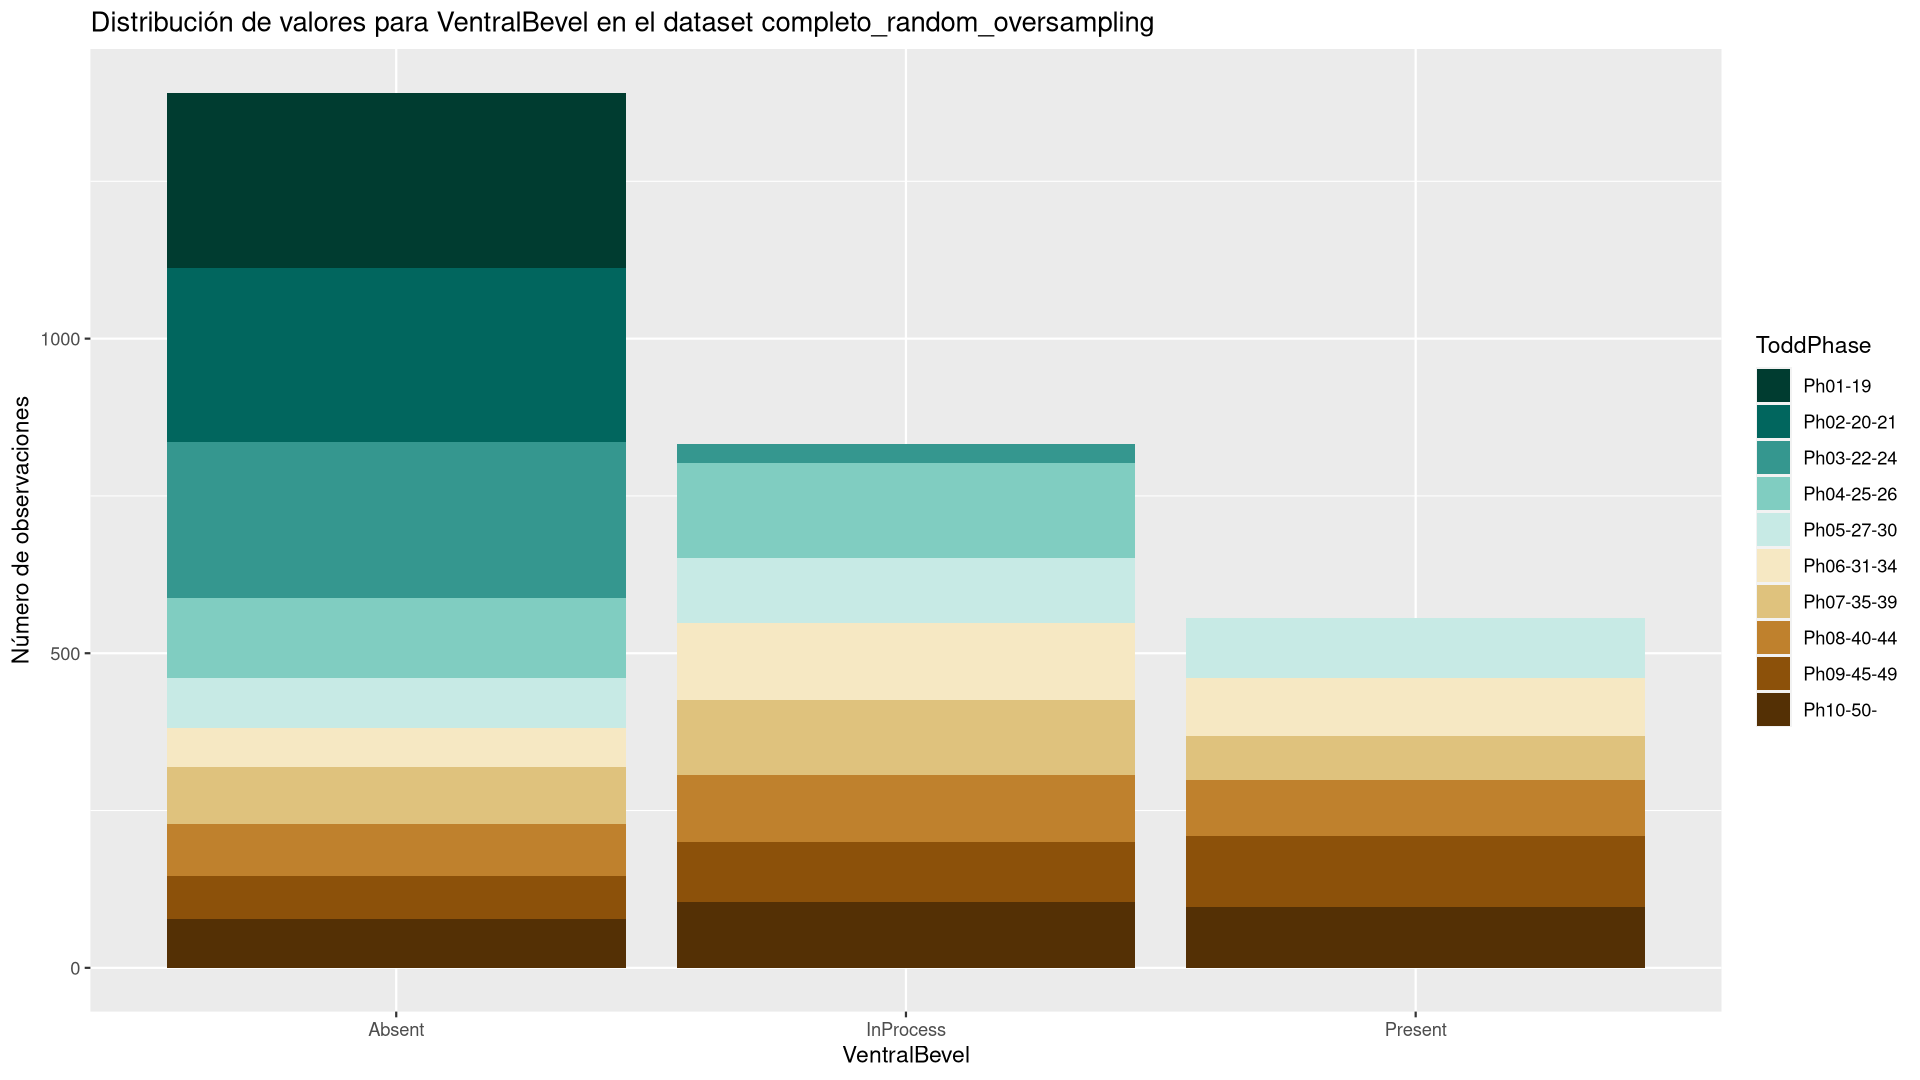
\includegraphics[width = \textwidth]{conjunto_random_oversampling/densidad_VentralBevel_completo_random_oversampling.png}
	\caption{Distribución de los valores de VentralBevel en el conjunto de datos completo tras aplicar sobremuestreo aleatorio.}
	\label{fig:densidad_VentralBevel_completo_random_oversampling}
\end{figure}

\begin{figure}[H]
	\centering
	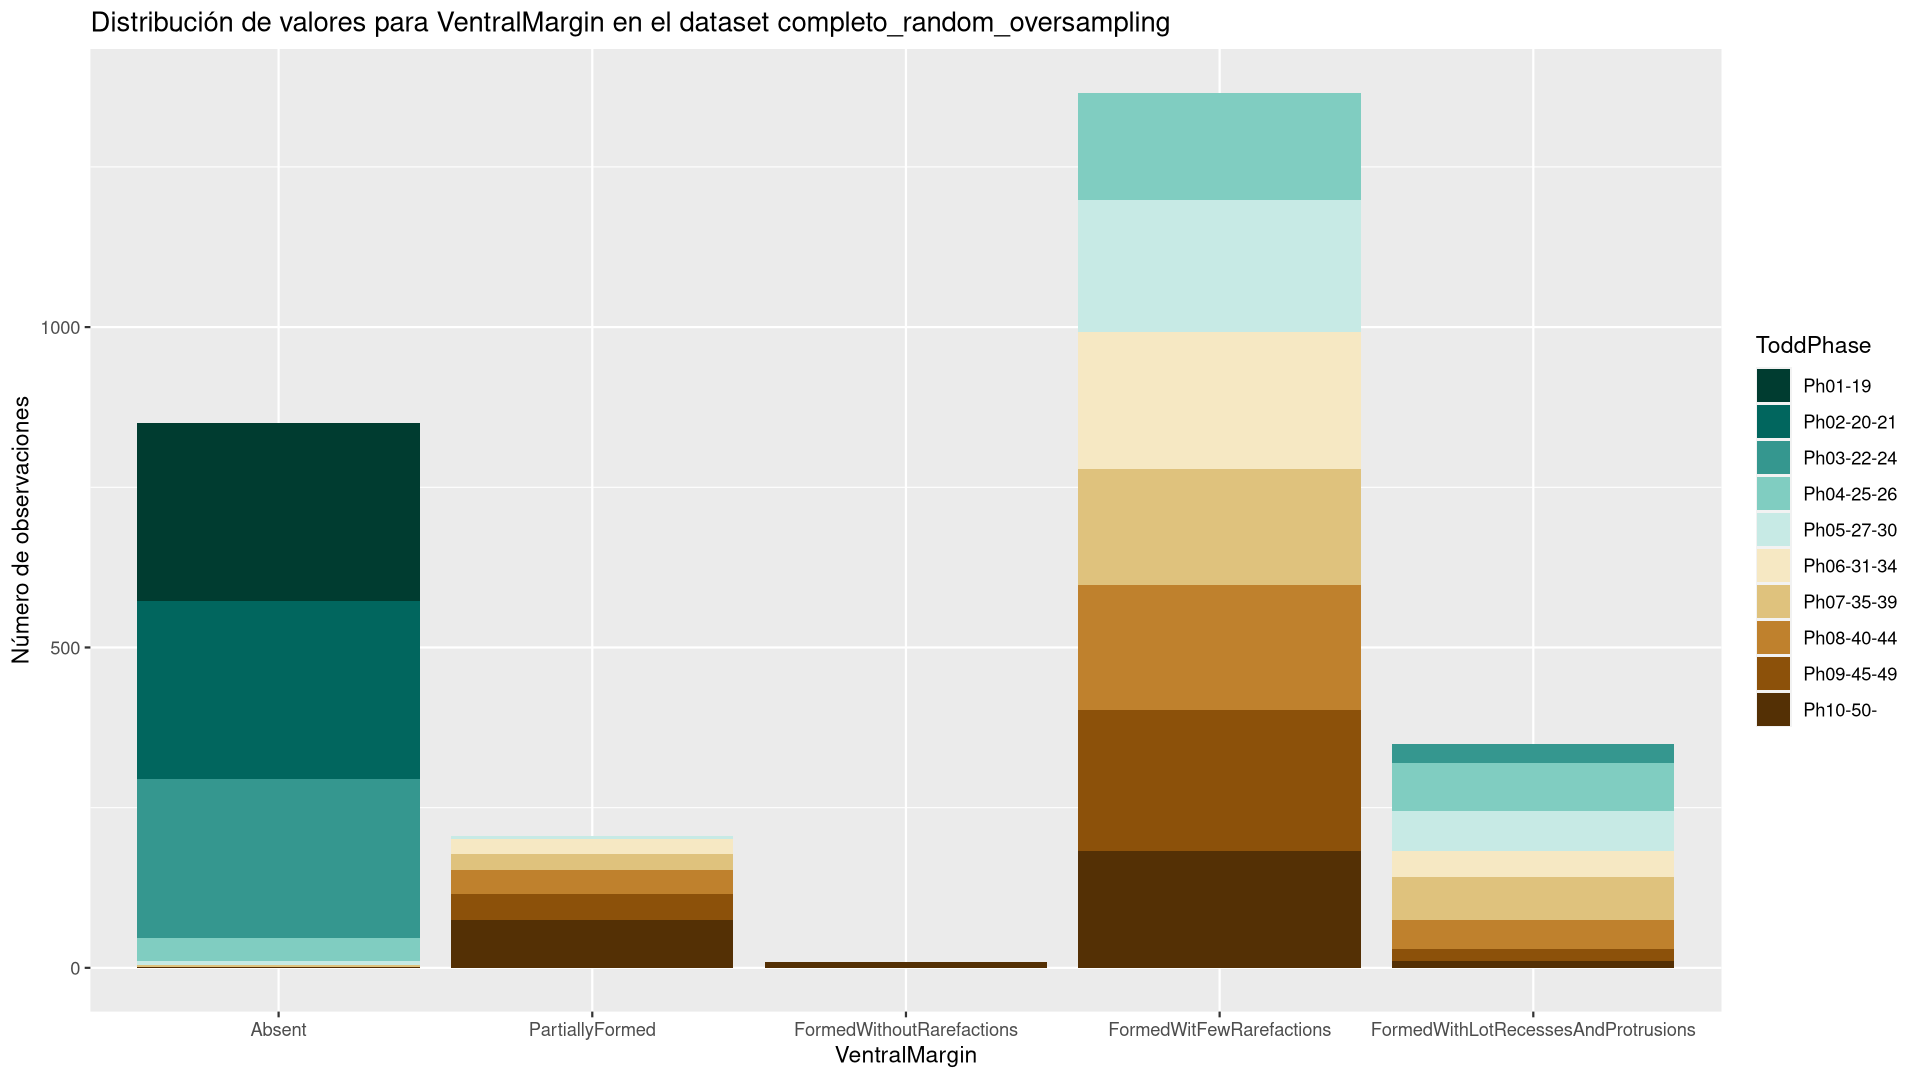
\includegraphics[width = \textwidth]{conjunto_random_oversampling/densidad_VentralMargin_completo_random_oversampling.png}
	\caption{Distribución de los valores de VentralMargin en el conjunto de datos completo tras aplicar sobremuestreo aleatorio.}
	\label{fig:densidad_VentralMargin_completo_random_oversampling}
\end{figure}


\subsubsection{Análisis del conjunto completo tras aplicar SMOTE}

\begin{figure}[H]
	\centering
	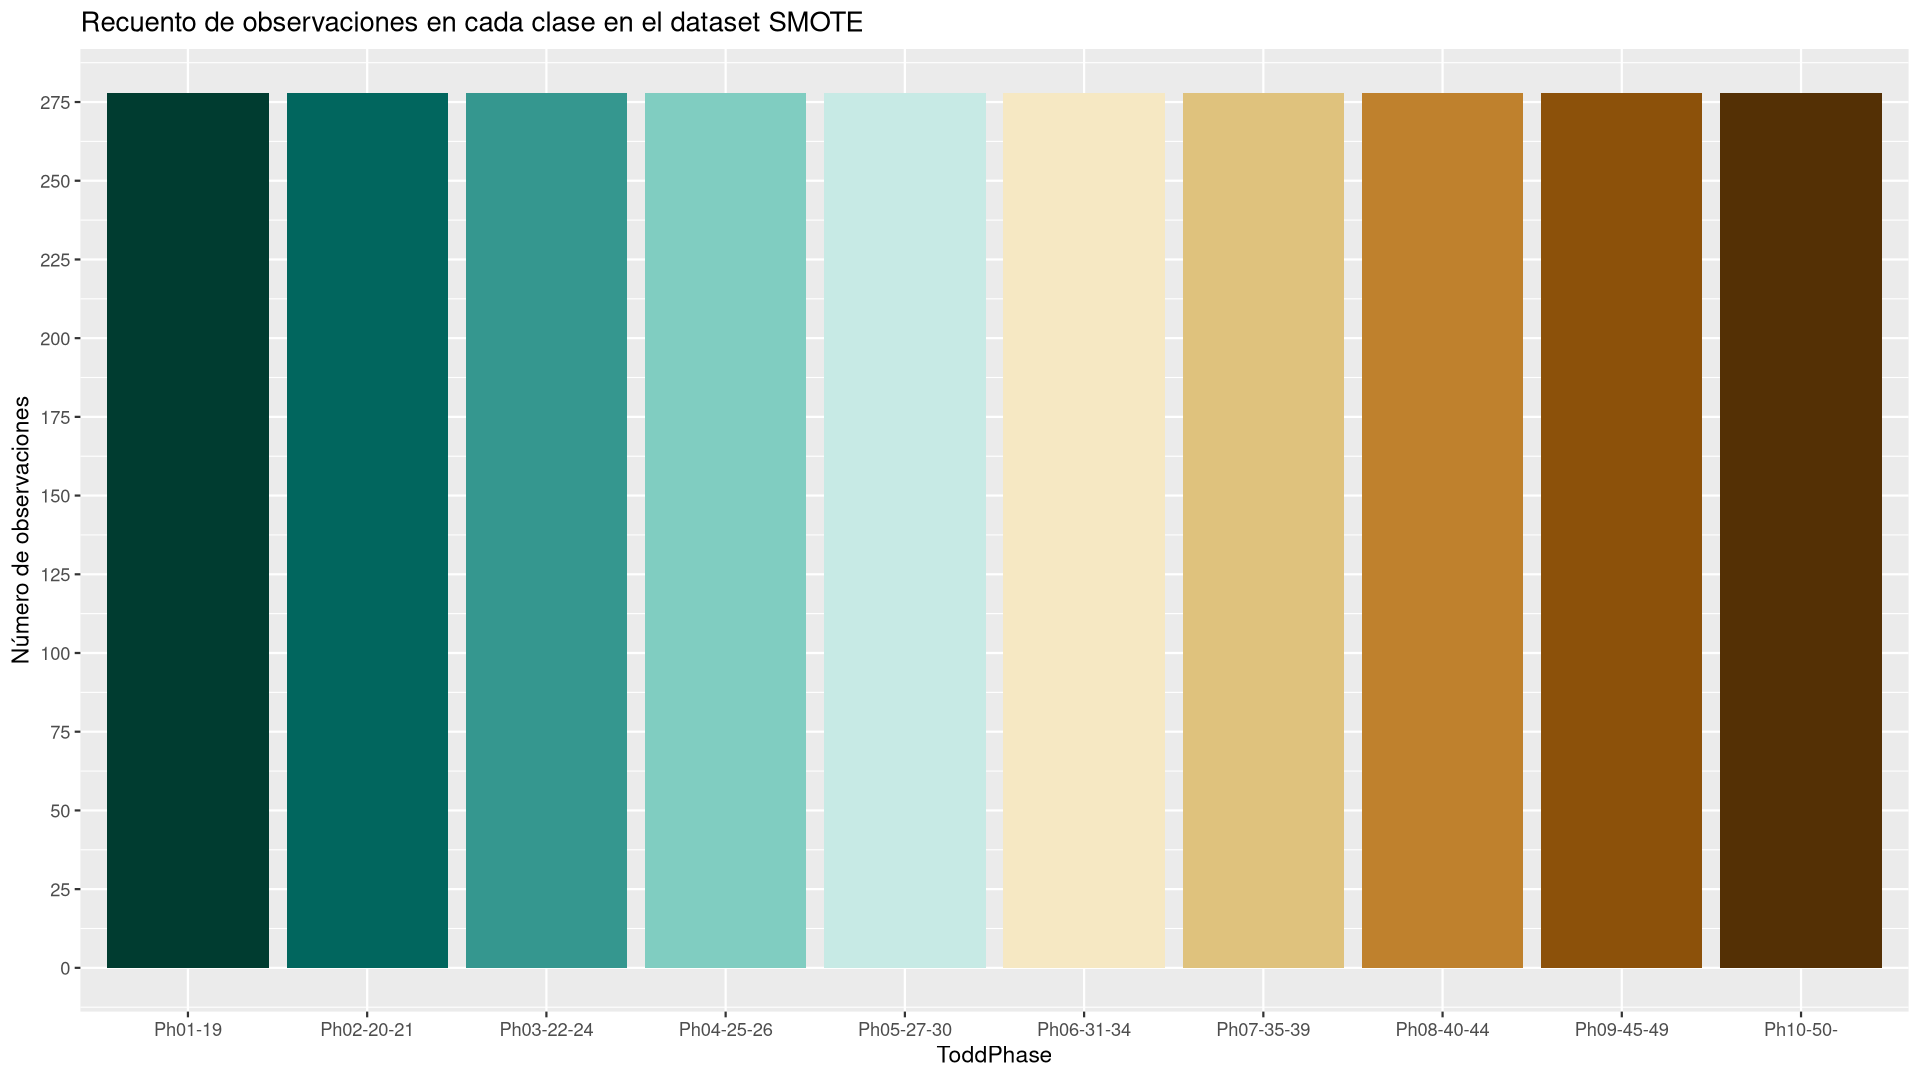
\includegraphics[width = \textwidth]{conjunto_datos_smote/distribucion_clases_SMOTE.png}
	\caption{Número de datos por cada fase propuesta por Todd con el conjunto de datos completo.}
	\label{fig:conteo_c_smote}
\end{figure}

Como era de esperar, claramente se han balanceado el número de observaciones de cada clase, como era de esperar. Vamos a ver si la introducción de observaciones sintéticas ha introducido ruido o algún problema en el conjunto de datos.


\begin{figure}[H]
	\centering
	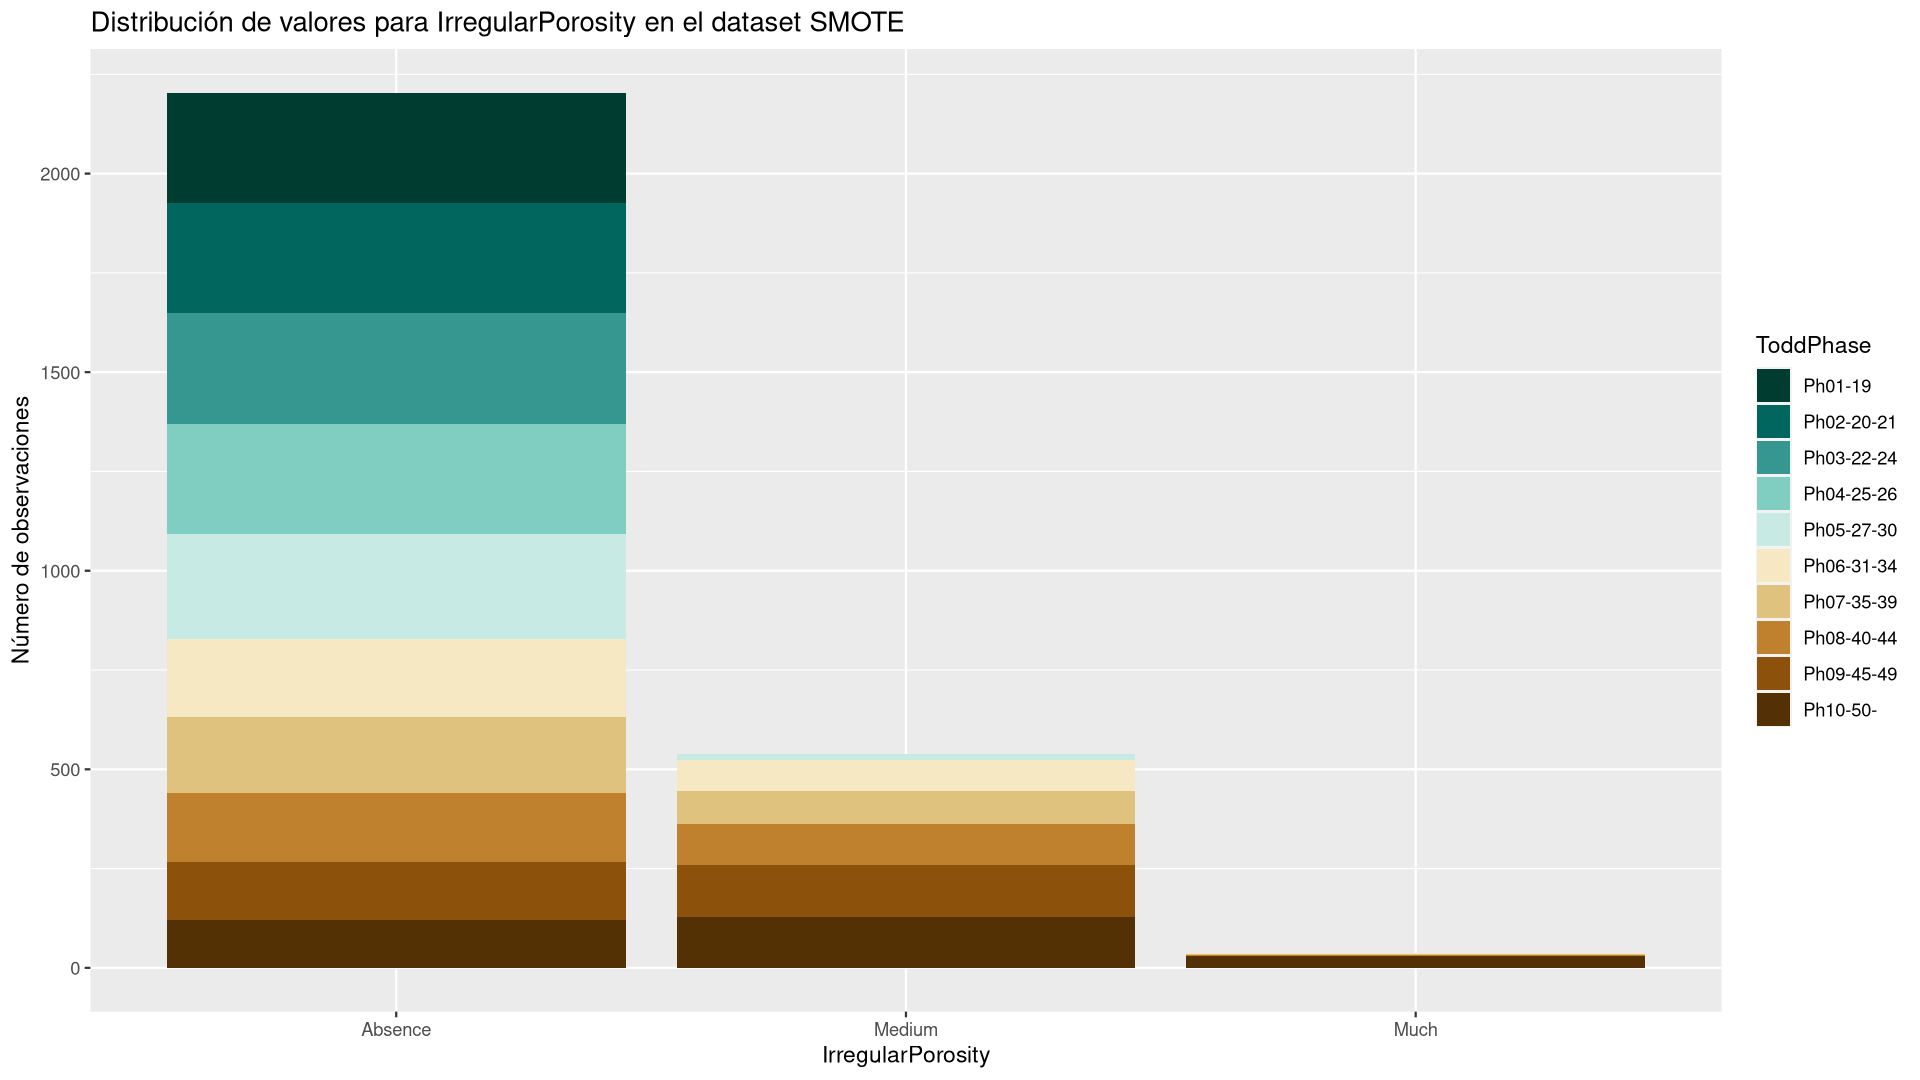
\includegraphics[width = \textwidth]{conjunto_datos_smote/densidad_IrregularPorosity_SMOTE.png}
	\caption{Distribución de los valores de IrregularPorosity en el conjunto de datos completo.}
	\label{fig:densidad_IrregularPorosity_SMOTE}
\end{figure}

Para \texttt{IrregularPorosity} vemos como ahora para el valor \texttt{Absence} todas las fases tienen un número de observaciones similar, cuando antes aunque existían observaciones de todas las clases con este valor, las de la fase cuatro al ser tan minoritaria podría pasar desapercibida. Por otro lado vemos como el número de observaciones con valor \texttt{Medium} casi se ha duplicado, pero manteniendo las observaciones que vimos anteriormente, este valor solo lo toman observaciones de fases altas. Esto último también ha ocurrido con el valor \texttt{Much}.

\begin{figure}[H]
	\centering
	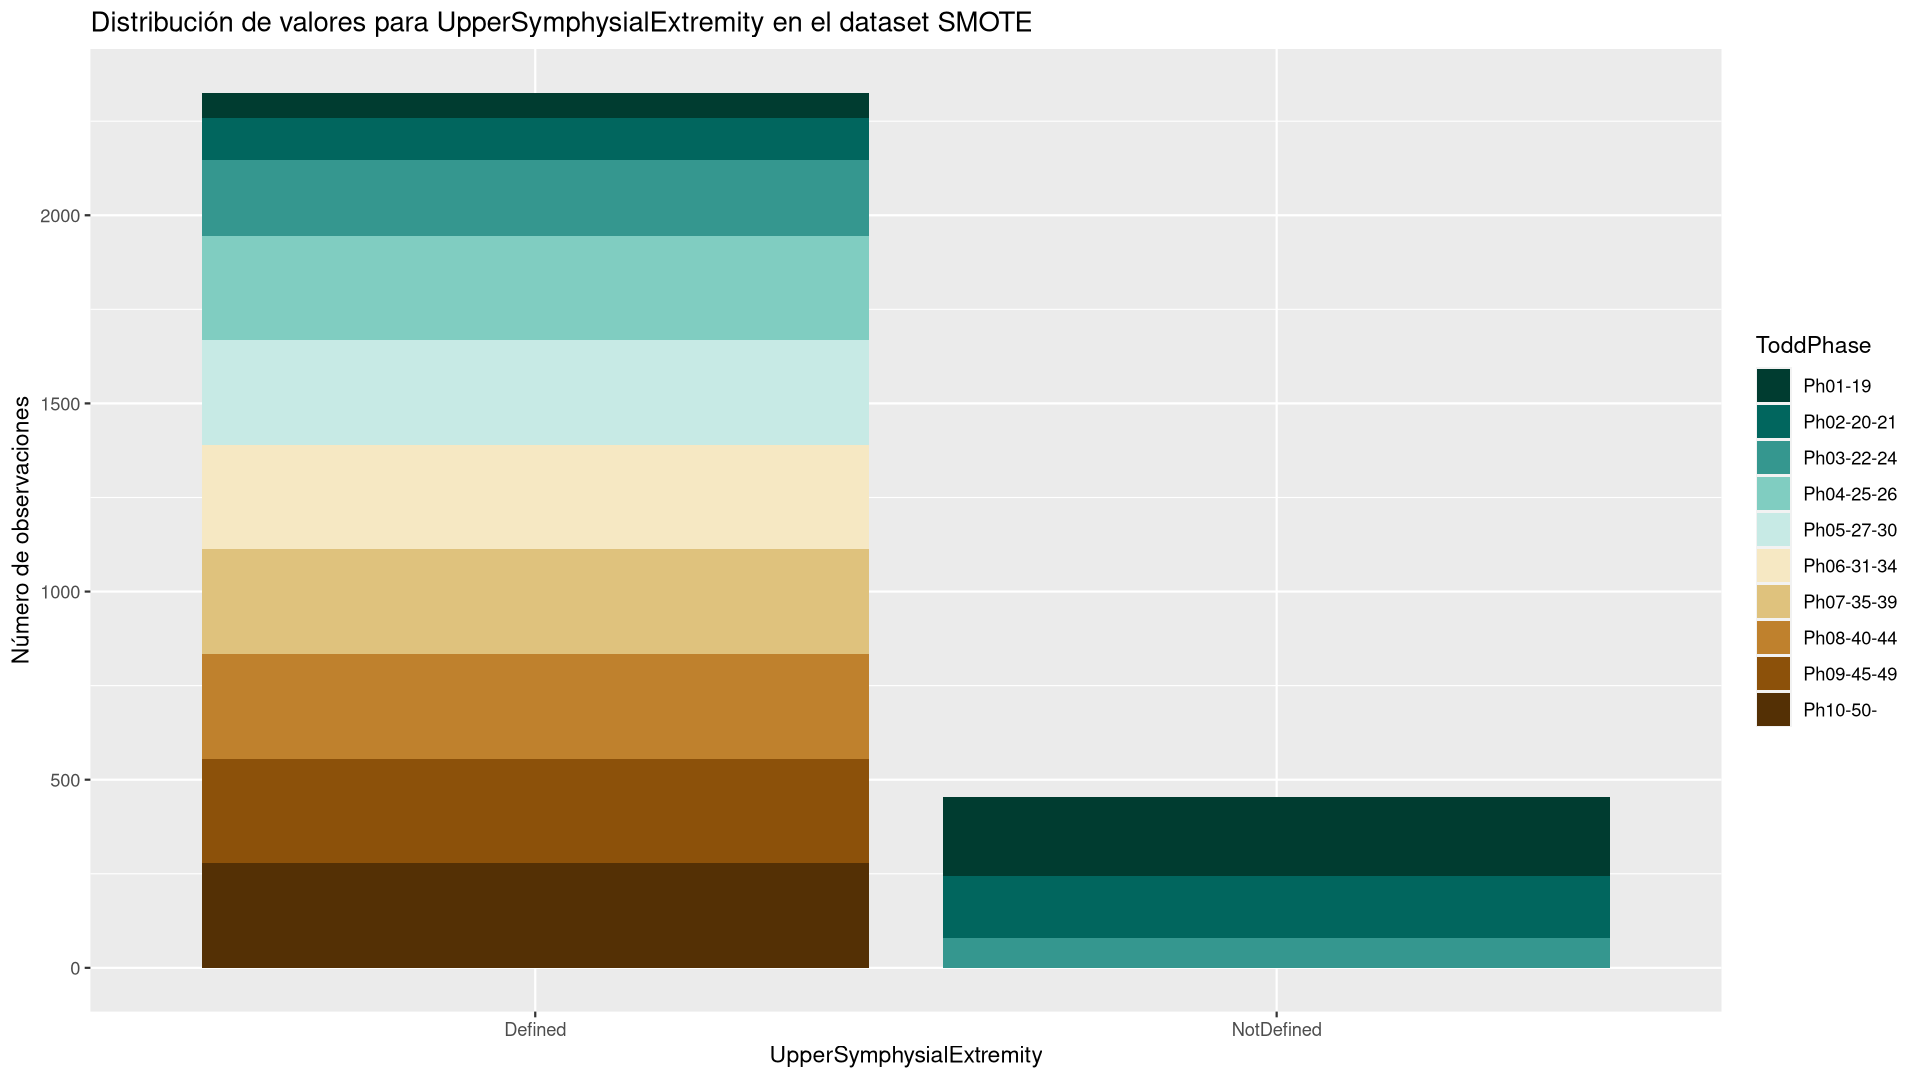
\includegraphics[width = \textwidth]{conjunto_datos_smote/densidad_UpperSymphysialExtremity_SMOTE.png}
	\caption{Distribución de los valores de UpperSymphysialExtremity en el conjunto de datos completo.}
	\label{fig:densidad_UpperSymphysialExtremity_SMOTE}
\end{figure}

Con \texttt{UpperSymphysialExtremity} de nuevo vuelve a ocurrir que la distribución de las fases para valores de \texttt{Defined} se equilibra, al añadir más instancias de las clases minoritarias, sin embargo hay que tener en cuenta que cuanto más baja es la fase, menos observaciones aparecen y más pasan al valor \texttt{NotDefined}, luego la aplicación de SMOTE nos ha confirmado que aunque algunas observaciones de fases bajas toman el valor de \texttt{Defined}, esto no es lo común y suelen tomar el valor de \texttt{NotDefined}.

\begin{figure}[H]
	\centering
	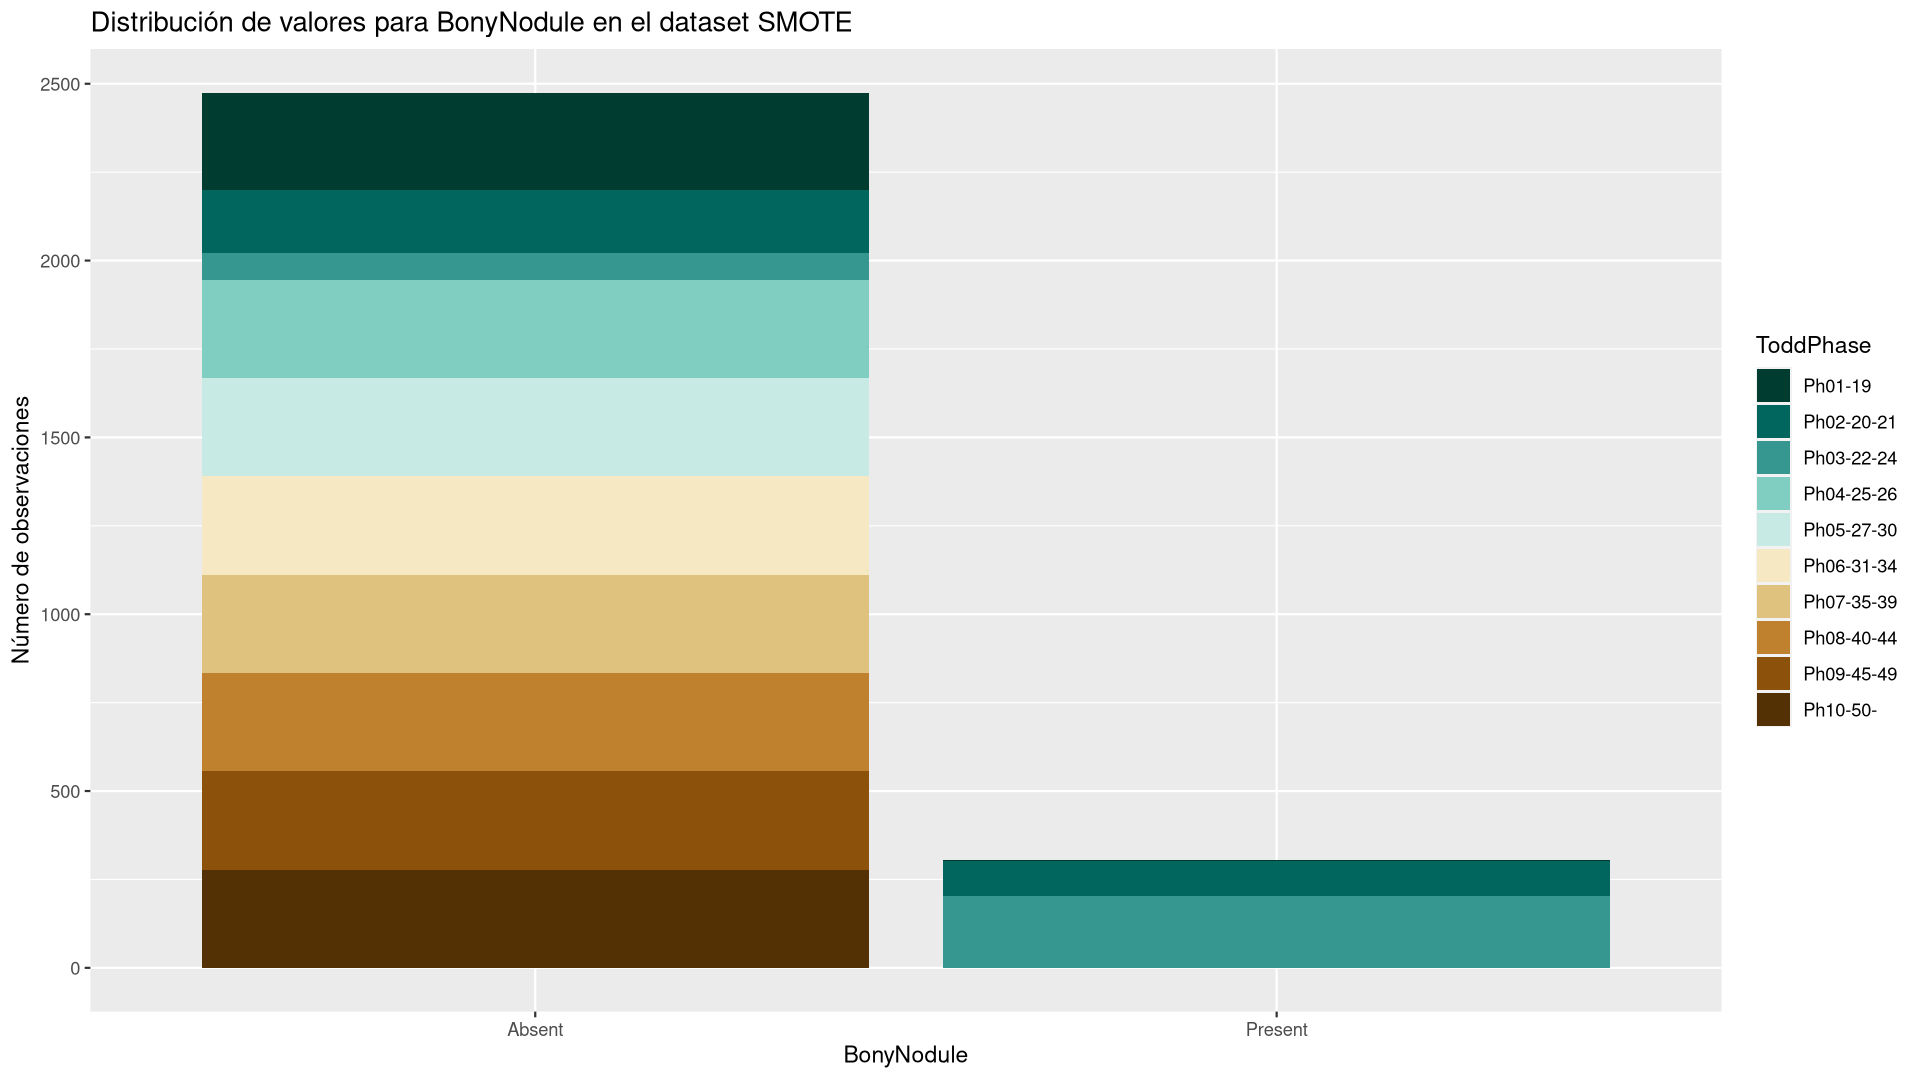
\includegraphics[width = \textwidth]{conjunto_datos_smote/densidad_BonyNodule_SMOTE.png}
	\caption{Distribución de los valores de BonyNodule en el conjunto de datos completo.}
	\label{fig:densidad_BonyNodule_SMOTE}
\end{figure}

En el caso de \texttt{BonyNodule} vuelve a ocurrir lo mismo que con \texttt{UpperSymphysialExtremity} pero con la segunda y tercera fase.


\begin{figure}[H]
	\centering
	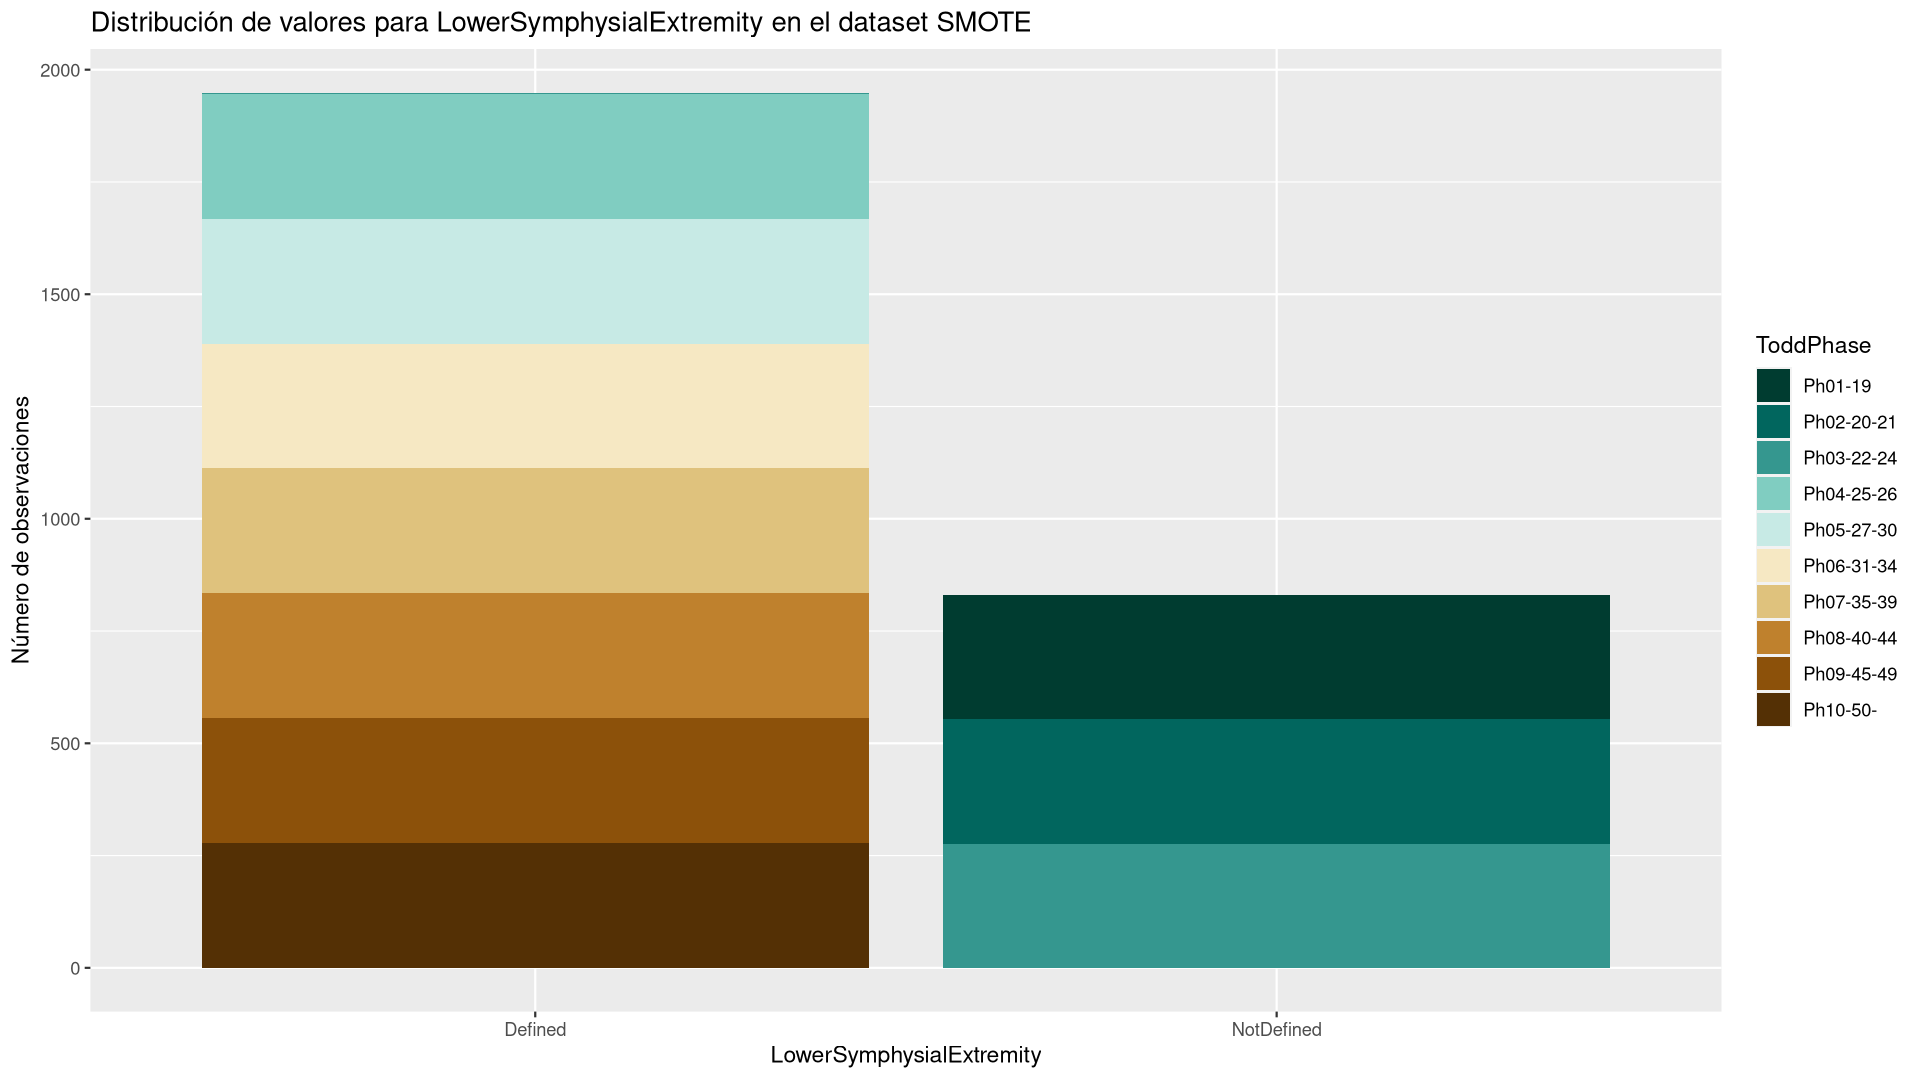
\includegraphics[width = \textwidth]{conjunto_datos_smote/densidad_LowerSymphysialExtremity_SMOTE.png}
	\caption{Distribución de los valores de LowerSymphysialExtremity en el conjunto de datos completo.}
	\label{fig:densidad_LowerSymphysialExtremity_SMOTE}
\end{figure}

Con \texttt{LowerSymphysialExtremity} se vuelve a repetir lo comentado anteriormente, pero en este caso dejando todavía más claro que el valor \texttt{NotDefined} solo lo toman valores de la primera y segunda fase, mientras que existe algo de solape entre \texttt{Defined} y \texttt{NotDefined} en la tercera fase, y de la cuarta fase en adelante siempre toma el valor de \texttt{Defined}.

\begin{figure}[H]
	\centering
	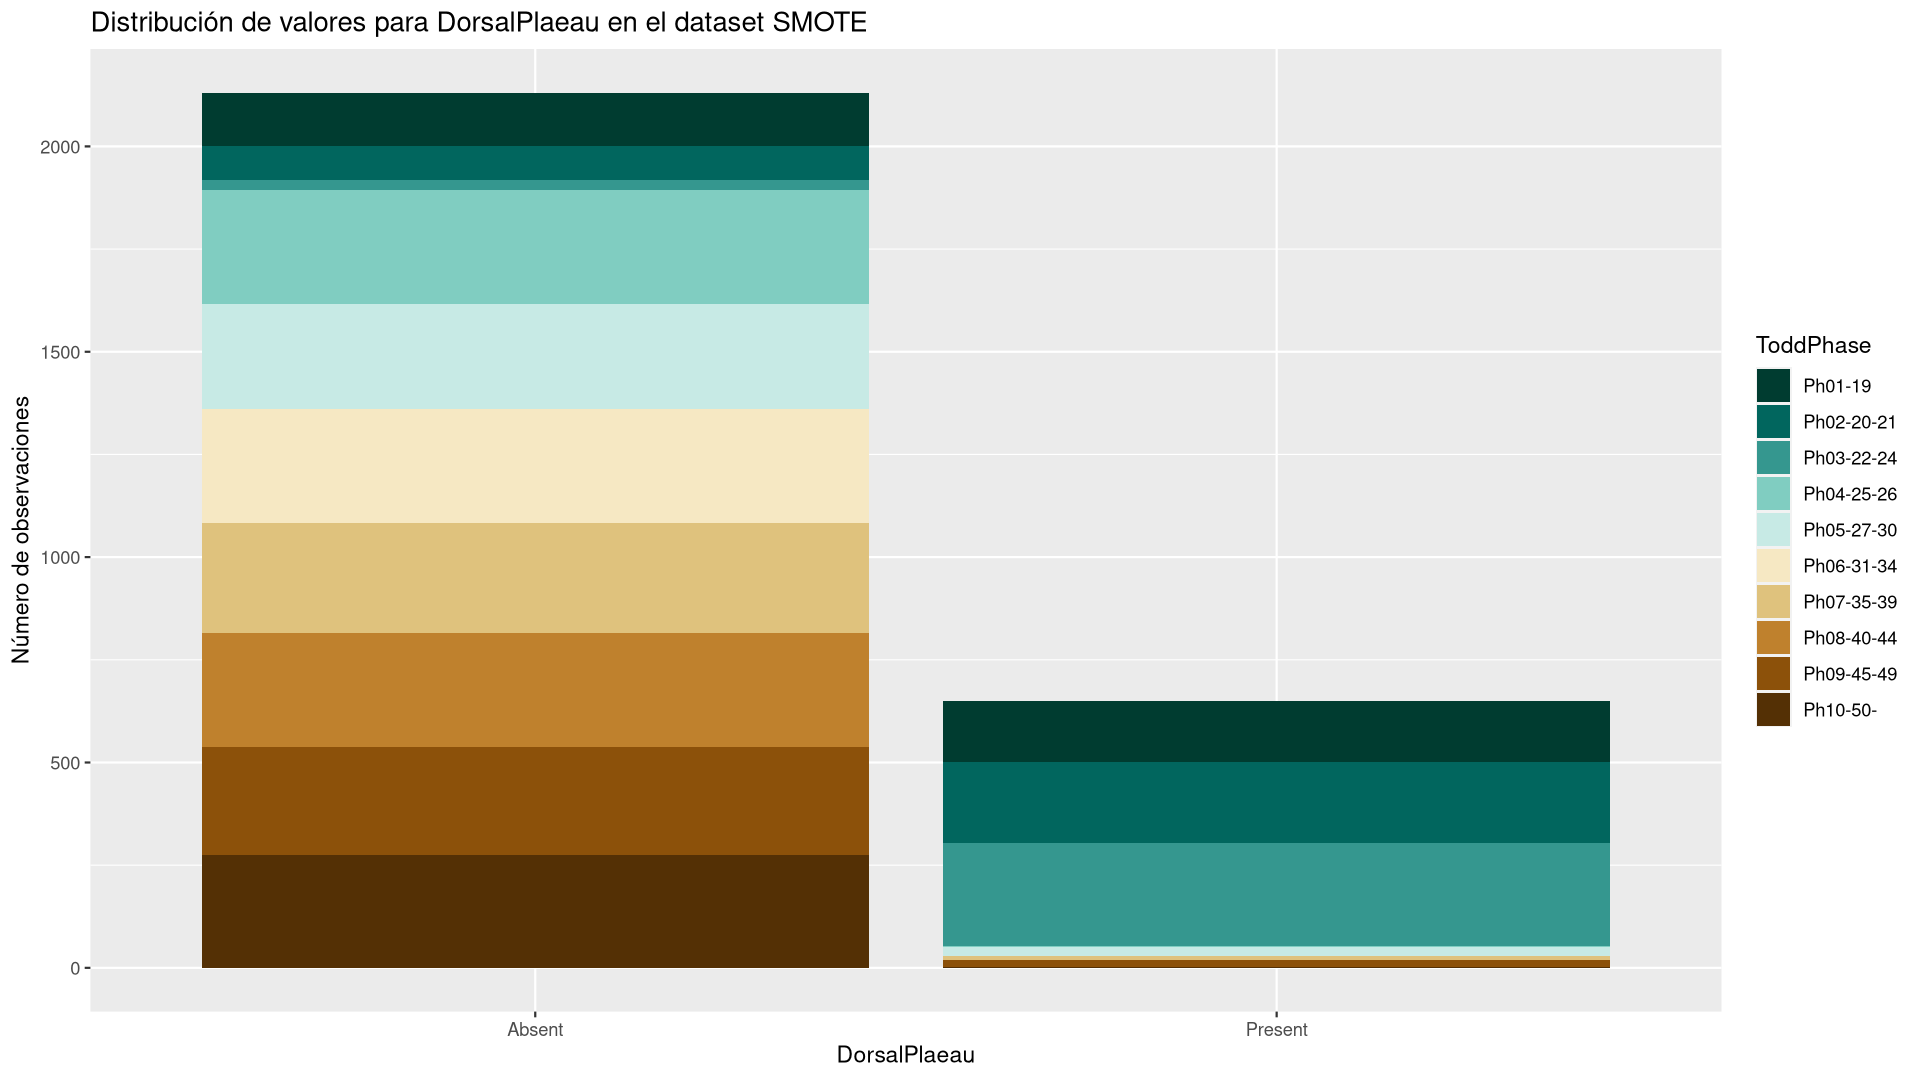
\includegraphics[width = \textwidth]{conjunto_datos_smote/densidad_DorsalPlaeau_SMOTE.png}
	\caption{Distribución de los valores de DorsalPlaeau en el conjunto de datos completo.}
	\label{fig:densidad_DorsalPlaeau_SMOTE}
\end{figure}

Observando como se ha comportado SMOTE con \texttt{DorsalPlaeau} podemos sacar unas conclusiones más interesantes. Al principio parecía que este predictor no aportaba información debido a que tanto con \texttt{Absent} como con \texttt{Present} había observaciones de todas las clases, sin embargo tras aplicar SMOTE podemos ver como ha encontrado muchos más vecinos de las tres primeras clases con valor \texttt{Present} que con \texttt{Absent}, mientras que el resto de clases no ha encontrado vecinos con los que aumentar el número de observaciones con \texttt{Present}, haciendo que ahora este valor sea mayormente indicador de que la observación se encuentra en las tres primeras fases.

\begin{figure}[H]
	\centering
	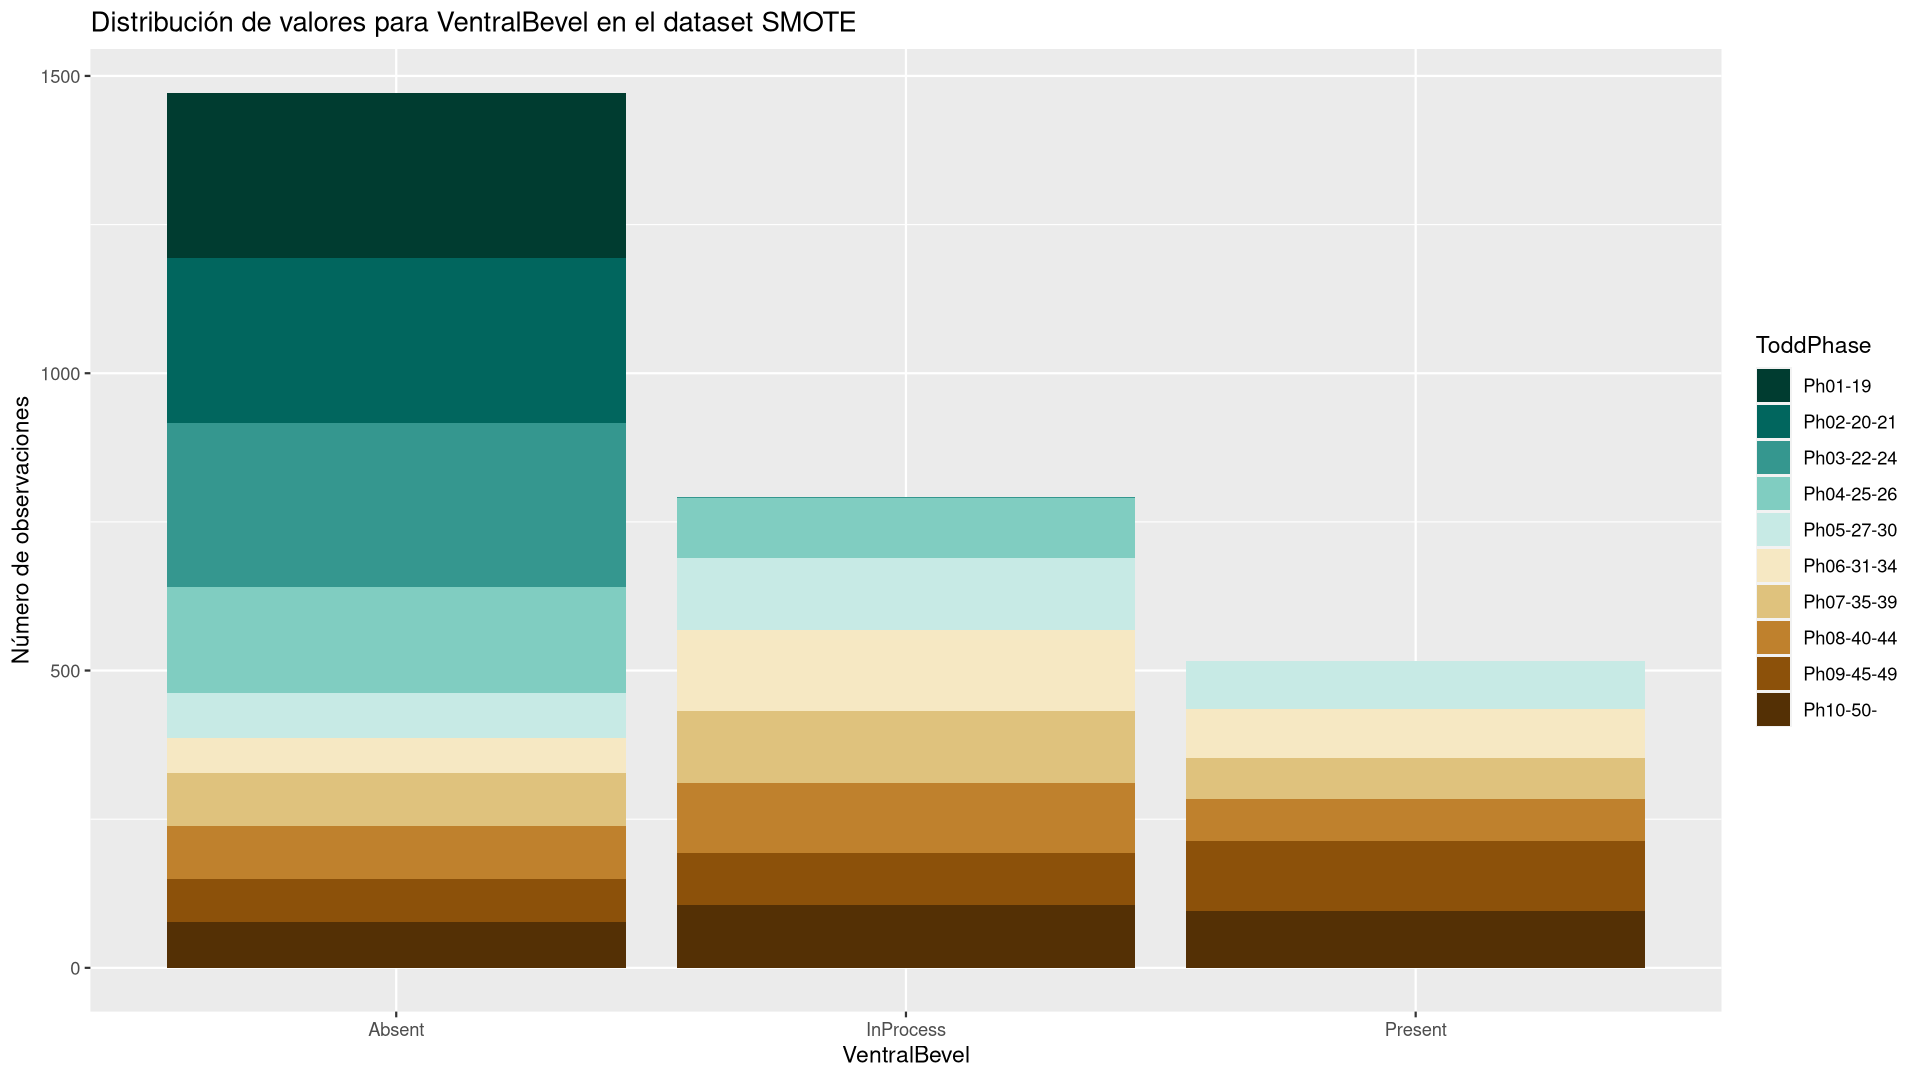
\includegraphics[width = \textwidth]{conjunto_datos_smote/densidad_VentralBevel_SMOTE.png}
	\caption{Distribución de los valores de VentralBevel en el conjunto de datos completo.}
	\label{fig:densidad_VentralBevel_SMOTE}
\end{figure}

Para \texttt{VentralBevel}, como con otros predictores, con SMOTE ha mantenido lo que observamos al analizar los datos originales. Si se toma el valor de \texttt{InProcess} y en especial \texttt{Present} es indicador de que la observación se trata de una fase alta.


\begin{figure}[H]
	\centering
	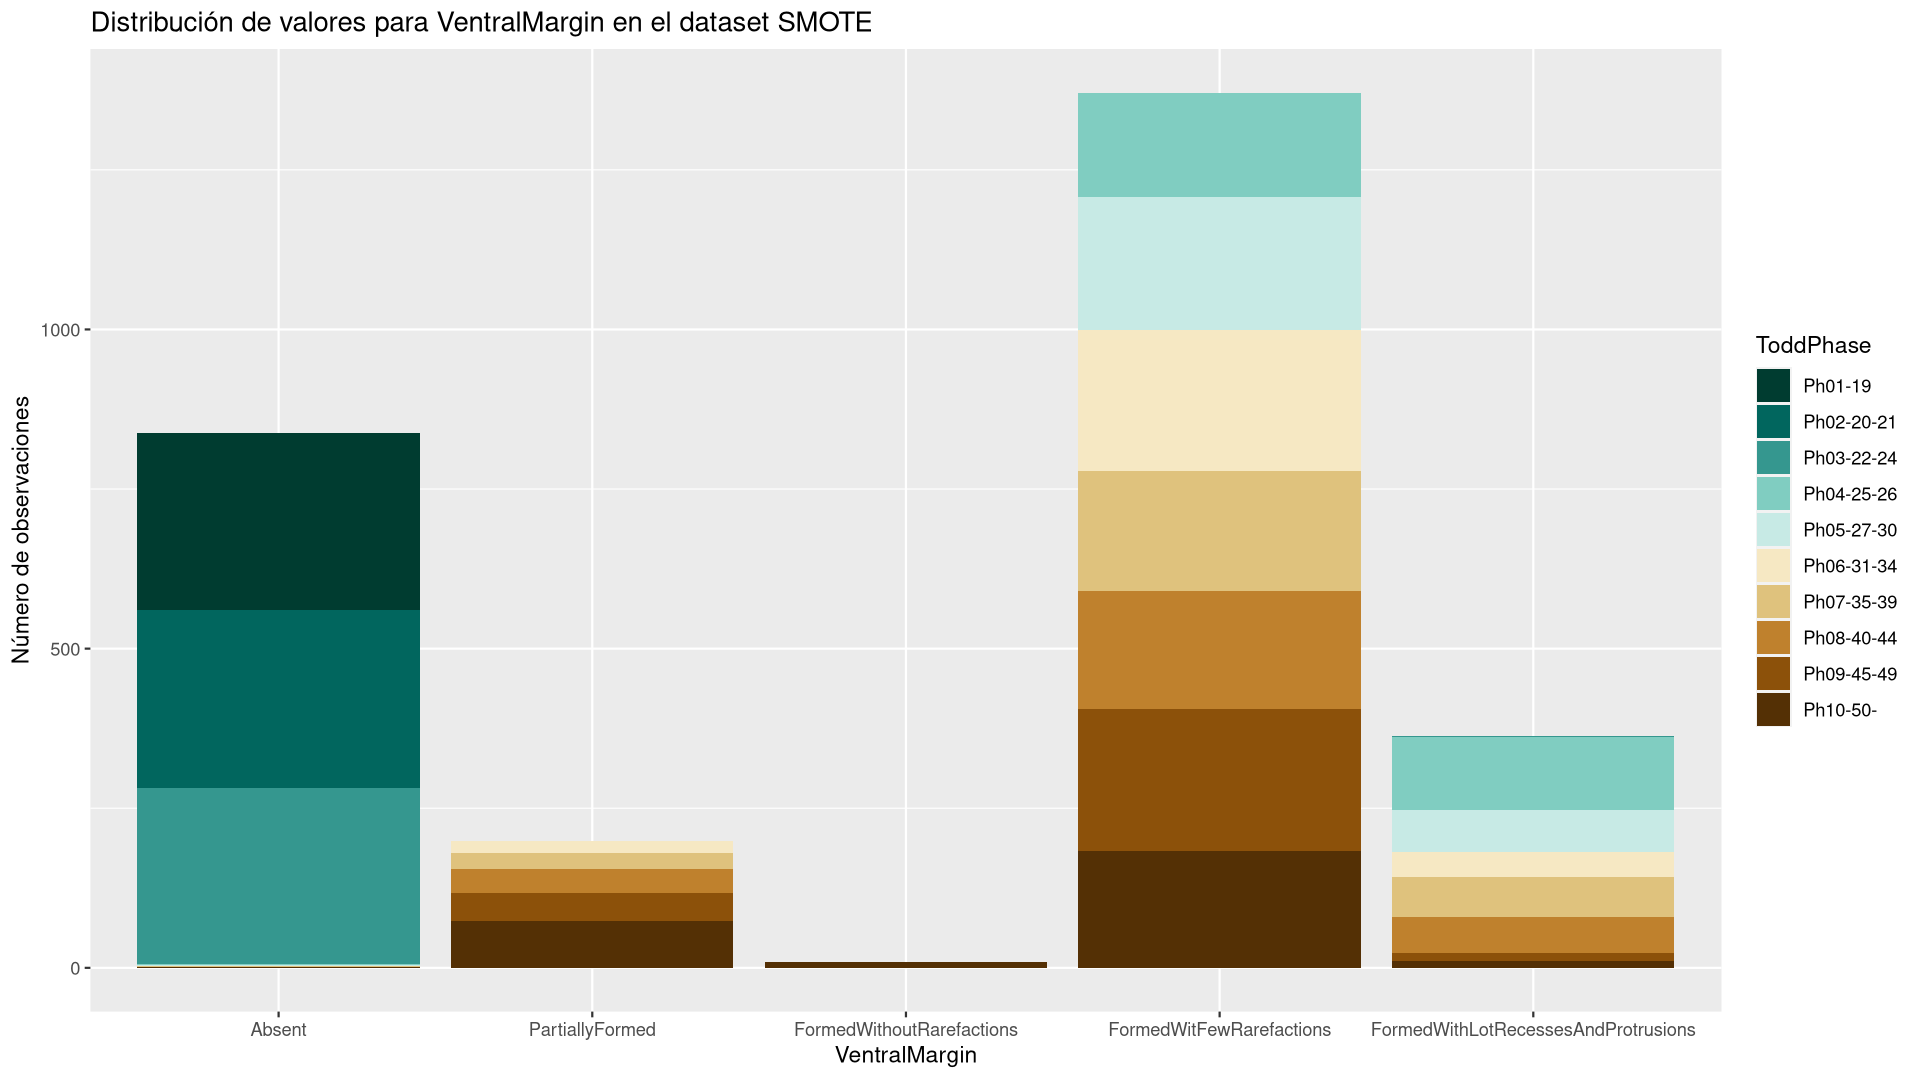
\includegraphics[width = \textwidth]{conjunto_datos_smote/densidad_VentralMargin_SMOTE.png}
	\caption{Distribución de los valores de VentralMargin en el conjunto de datos completo.}
	\label{fig:densidad_VentralMargin_SMOTE}
\end{figure}

Por último, para la variable \texttt{VentralMargin} que apenas se ha modificado la distribución, como podemos ver, simplemente se equilibran las clases para los distintos valores, aunque podemos ver que claramente sigue existiendo algunos valores que solo toman ciertas clases, como \texttt{Absent}, que principalmente se trata de fases tempranas, o \texttt{PartiallyFormed}, que mayormente son observaciones de las últimas fases.

\newpage


\subsubsection{Análisis del conjunto completo tras aplicar BorderlineSMOTE}

Debido a que las soluciones para BorderlineSMOTE son muy parecidas a nivel gráfico que las de SMOTE, no se han añadido las imágenes para no extender de forma innecesaria el análisis, debido a que se sacarían las mismas conclusiones.

Lo importante de aplicar este algoritmo sería si las observaciones generadas realmente se encuentran en una zona crucial de la frontera de decisión, sin embargo esto no lo podemos observar de forma gráfica al contar con demasiadas dimensiones.

\subsubsection{Conclusiones de la aplicación de sobremuestreo}


Como conclusiones comentar que, a priori, con este pequeño análisis de datos, parece que estas técnicas de sobremuestreo pueden ayudar a la hora de entrenar el modelo.

La aplicación de estas técnicas nos puede ayudar a reafirmar la utilidad de ciertos valores para decidir la fase o al menos acotarla, por lo que podría disminuir el sesgo del modelo sin haber añadido información errónea. Además, con contar con la técnica básica de sobremuestreo aleatorio, tenemos un caso donde no hemos introducido observaciones generadas de forma sintética (evitando añadir ruido e información errónea) pero solucionando el problema del balanceo de clases al lanzar el conjunto de experimentos.



\newpage
